\documentclass[twoside]{book}

% Packages required by doxygen
\usepackage{fixltx2e}
\usepackage{calc}
\usepackage{doxygen}
\usepackage[export]{adjustbox} % also loads graphicx
\usepackage{graphicx}
\usepackage[utf8]{inputenc}
\usepackage{makeidx}
\usepackage{multicol}
\usepackage{multirow}
\PassOptionsToPackage{warn}{textcomp}
\usepackage{textcomp}
\usepackage[nointegrals]{wasysym}
\usepackage[table]{xcolor}

% Font selection
\usepackage[T1]{fontenc}
\usepackage[scaled=.90]{helvet}
\usepackage{courier}
\usepackage{amssymb}
\usepackage{sectsty}
\renewcommand{\familydefault}{\sfdefault}
\allsectionsfont{%
  \fontseries{bc}\selectfont%
  \color{darkgray}%
}
\renewcommand{\DoxyLabelFont}{%
  \fontseries{bc}\selectfont%
  \color{darkgray}%
}
\newcommand{\+}{\discretionary{\mbox{\scriptsize$\hookleftarrow$}}{}{}}

% Page & text layout
\usepackage{geometry}
\geometry{%
  a4paper,%
  top=2.5cm,%
  bottom=2.5cm,%
  left=2.5cm,%
  right=2.5cm%
}
\tolerance=750
\hfuzz=15pt
\hbadness=750
\setlength{\emergencystretch}{15pt}
\setlength{\parindent}{0cm}
\setlength{\parskip}{3ex plus 2ex minus 2ex}
\makeatletter
\renewcommand{\paragraph}{%
  \@startsection{paragraph}{4}{0ex}{-1.0ex}{1.0ex}{%
    \normalfont\normalsize\bfseries\SS@parafont%
  }%
}
\renewcommand{\subparagraph}{%
  \@startsection{subparagraph}{5}{0ex}{-1.0ex}{1.0ex}{%
    \normalfont\normalsize\bfseries\SS@subparafont%
  }%
}
\makeatother

% Headers & footers
\usepackage{fancyhdr}
\pagestyle{fancyplain}
\fancyhead[LE]{\fancyplain{}{\bfseries\thepage}}
\fancyhead[CE]{\fancyplain{}{}}
\fancyhead[RE]{\fancyplain{}{\bfseries\leftmark}}
\fancyhead[LO]{\fancyplain{}{\bfseries\rightmark}}
\fancyhead[CO]{\fancyplain{}{}}
\fancyhead[RO]{\fancyplain{}{\bfseries\thepage}}
\fancyfoot[LE]{\fancyplain{}{}}
\fancyfoot[CE]{\fancyplain{}{}}
\fancyfoot[RE]{\fancyplain{}{\bfseries\scriptsize Generated by Doxygen }}
\fancyfoot[LO]{\fancyplain{}{\bfseries\scriptsize Generated by Doxygen }}
\fancyfoot[CO]{\fancyplain{}{}}
\fancyfoot[RO]{\fancyplain{}{}}
\renewcommand{\footrulewidth}{0.4pt}
\renewcommand{\chaptermark}[1]{%
  \markboth{#1}{}%
}
\renewcommand{\sectionmark}[1]{%
  \markright{\thesection\ #1}%
}

% Indices & bibliography
\usepackage{natbib}
\usepackage[titles]{tocloft}
\setcounter{tocdepth}{3}
\setcounter{secnumdepth}{5}
\makeindex

% Hyperlinks (required, but should be loaded last)
\usepackage{ifpdf}
\ifpdf
  \usepackage[pdftex,pagebackref=true]{hyperref}
\else
  \usepackage[ps2pdf,pagebackref=true]{hyperref}
\fi
\hypersetup{%
  colorlinks=true,%
  linkcolor=blue,%
  citecolor=blue,%
  unicode%
}

% Custom commands
\newcommand{\clearemptydoublepage}{%
  \newpage{\pagestyle{empty}\cleardoublepage}%
}

\usepackage{caption}
\captionsetup{labelsep=space,justification=centering,font={bf},singlelinecheck=off,skip=4pt,position=top}

%===== C O N T E N T S =====

\begin{document}

% Titlepage & ToC
\hypersetup{pageanchor=false,
             bookmarksnumbered=true,
             pdfencoding=unicode
            }
\pagenumbering{roman}
\begin{titlepage}
\vspace*{7cm}
\begin{center}%
{\Large ln\+\_\+space }\\
\vspace*{1cm}
{\large Generated by Doxygen 1.8.11}\\
\end{center}
\end{titlepage}
\clearemptydoublepage
\tableofcontents
\clearemptydoublepage
\pagenumbering{arabic}
\hypersetup{pageanchor=true}

%--- Begin generated contents ---
\chapter{Logarithmic\+\_\+\+Strain\+\_\+\+Space-\/dealii}
\label{md_README}
\hypertarget{md_README}{}
C++ code using the deal.\+ii library for the transformation into the logarithmic strain space

(also available for Fortran, but not yet documented and uploaded)

\subsection*{The goal/\+When to use this code}

The logarithmic strain space (herein often abbreviated as ln-\/space) is a very simple (in terms of the application) way to apply small strain material models to finite strains. So, in case you have a small strain model that you would like to apply to applications exposed to large deformations/finite strains, the ln-\/space it probably the easiest way to achieve this.

All you need are three steps as schematically (simplified) shown in the figure\+:
\begin{DoxyEnumerate}
\item Pre-\/processing from the world of finite strains into the logarithmic strain space
\item Calling your small strain model with the Hencky strain computed in the pre-\/processing
\item Post-\/processing the computed stress and tangent(s) by transforming them from the ln-\/space back into the real world. And the best is, steps 1 and 3 are always the same (copy-\/paste) and the second step is the same as done for the small strain implementation.
\end{DoxyEnumerate}



Drawbacks?

Especially step 3, the post-\/processing is expensive independent of your material model. So, as far as efficiency is concerned, a simple material model utilising the ln-\/space is most certainly slower, than its derived finite strain equivalent (a model that was developed for finite strains). However, for complicated material models it can be faster to use the small strain model in the ln-\/space, instead of a finite strain equivalent (and it requires no further derivations/development to get from small to finite strains). Another disadvantage, is the limitation to small elastic strains. The latter is usually satisfied for metal forming and similar applications, where elastic strain are small and large plastic strain occur.

\subsection*{Background}

\begin{DoxyRefDesc}{Todo}
\item[\hyperlink{todo__todo000001}{Todo}]add some equations\end{DoxyRefDesc}


The transformation consists of three steps. First, we transform the deformation gradient {\ttfamily F} into the logarithmic strain space (ln-\/space) and obtain the Hencky strain (preprocessing). Secondly, the standard small strain material model is called using the Hencky strain and the usual history. The outcome is the stress measure {\ttfamily T} and the fourth order tangent {\ttfamily C}. Finally, we transform the stress and tangent modulus back from the logarithmic strain space to obtain e.\+g. the Second Piola-\/\+Kirchhoff stress tensor {\ttfamily S}and the Lagrangian tangent modulus {\ttfamily L} (postprocessing).

\subsection*{Interface/\+How to use this code}


\begin{DoxyItemize}
\item Add the \hyperlink{classln__space}{ln\+\_\+space} header files (.h) and auxiliary functions from this repository to your working directory.
\item Include the header \char`\"{}ln\+\_\+space.\+h\char`\"{} in your code
\item Create an instance of the \hyperlink{classln__space}{ln\+\_\+space} class 
\begin{DoxyCode}
1 ln\_space<dim> ln\_space;
\end{DoxyCode}

\item Execute the preprocessing step using the deformation gradient as input 
\begin{DoxyCode}
1 ln\_space.pre\_ln(F);
\end{DoxyCode}

\item Get the Hencky strain {\ttfamily hencky\+\_\+strain} from the \hyperlink{classln__space}{ln\+\_\+space} and call your material model (e.\+g. elastoplasticity(...)) with the Hencky strain as the input strain 
\begin{DoxyCode}
1 SymmetricTensor<2,dim> hencky\_strain = ln\_space.hencky\_strain;
2 SymmetricTensor<4,3> tangent = elastoplasticity(/*input->*/ hencky\_strain, history, /*output->*/ T\_stress);
\end{DoxyCode}

\item Execute the postprocessing using the computed {\ttfamily T\+\_\+stress} and tangent as input 
\begin{DoxyCode}
1 ln\_space.post\_ln(T\_stress,tangent);
\end{DoxyCode}

\item Extract the Second Piola-\/\+Kirchhoff stress tensor {\ttfamily stress\+\_\+S} and the Lagrangian tangent modulus {\ttfamily L} 
\begin{DoxyCode}
1 SymmetricTensor<2,dim> stress\_S = ln\_space.second\_piola\_stress\_S;
2 SymmetricTensor<4,dim> L = ln\_space.C;
\end{DoxyCode}

\end{DoxyItemize}

\subsection*{The code/ A look under the hood}

The documentation for the ln-\/space code can be found here \href{https://jfriedlein.github.io/Logarithmic_Strain_Space-dealii/html/namespaceln__space.html}{\tt https\+://jfriedlein.\+github.\+io/\+Logarithmic\+\_\+\+Strain\+\_\+\+Space-\/dealii/html/namespaceln\+\_\+\+\_\+space.\+html}.

\begin{DoxyRefDesc}{Todo}
\item[\hyperlink{todo__todo000002}{Todo}]Create a proper mainpage instead of this namespace-\/thing\end{DoxyRefDesc}


\subsection*{References and Literature}


\begin{DoxyItemize}
\item papers on the algorithms\+:
\begin{DoxyItemize}
\item Miehe, C. and Lambrecht, M. (2001), Algorithms for computation of stresses and elasticity moduli in terms of Seth–\+Hill\textquotesingle{}s family of generalized strain tensors. Commun. Numer. Meth. Engng., 17\+: 337-\/353. doi\+:10.\+1002/cnm.404
\item Miehe, C. \& Apel, N. \& Lambrecht, M.. (2002). Anisotropic additive plasticity in the logarithmic strain space\+: Modular kinematic formulation and implementation based on incremental minimization principles for standard materials. Computer Methods in Applied Mechanics and Engineering -\/ C\+O\+M\+P\+UT M\+E\+T\+H\+OD A\+P\+PL M\+E\+CH E\+NG. 191. 5383-\/5425. 10.\+1016/\+S0045-\/7825(02)00438-\/3.
\end{DoxyItemize}
\item papers on the application\+:
\begin{DoxyItemize}
\item ...
\end{DoxyItemize}
\end{DoxyItemize}

\subsection*{To\+Do}


\begin{DoxyItemize}
\item rename variables, e.\+g. \textquotesingle{}C\textquotesingle{} should be lagrangian tangent ...
\item avoid directly accessing the member variables, use access functions instead, e.\+g. with const return values
\item merge the for-\/loops in the 2D pre\+\_\+ln
\item check which header files are needed
\item pack all needed external functions into an own auxiliary script (maybe requires namespace to avoid overloading)
\item add a remark on how to handle the 2D case (extract\+\_\+dim, ...)
\item add an intro text
\item complete the documentation (comments)
\item maybe add an example of a basic code calling the matmod with the ln-\/space (e.\+g. deal.\+ii example expanded to finite strains) 
\end{DoxyItemize}
\chapter{Todo List}
\label{todo}
\hypertarget{todo}{}

\begin{DoxyRefList}
\item[\label{todo__todo000001}%
\hypertarget{todo__todo000001}{}%
Page \hyperlink{md_README}{Logarithmic\+\_\+\+Strain\+\_\+\+Space-\/dealii} ]add some equations

Create a proper mainpage instead of this namespace-\/thing
\end{DoxyRefList}
\chapter{Class Index}
\section{Class List}
Here are the classes, structs, unions and interfaces with brief descriptions\+:\begin{DoxyCompactList}
\item\contentsline{section}{\hyperlink{classConstitutive__Laws_1_1Thermo__Elasto__Plastic}{Constitutive\+\_\+\+Laws\+::\+Thermo\+\_\+\+Elasto\+\_\+\+Plastic$<$ dim $>$} }{\pageref{classConstitutive__Laws_1_1Thermo__Elasto__Plastic}}{}
\end{DoxyCompactList}

\chapter{File Index}
\section{File List}
Here is a list of all files with brief descriptions\+:\begin{DoxyCompactList}
\item\contentsline{section}{\hyperlink{functions_8h}{functions.\+h} }{\pageref{functions_8h}}{}
\item\contentsline{section}{\hyperlink{ln__space_01pre__func__post_8h}{ln\+\_\+space pre\+\_\+func\+\_\+post.\+h} }{\pageref{ln__space_01pre__func__post_8h}}{}
\item\contentsline{section}{\hyperlink{ln__space_8h}{ln\+\_\+space.\+h} }{\pageref{ln__space_8h}}{}
\item\contentsline{section}{\hyperlink{mainpage_8h}{mainpage.\+h} }{\pageref{mainpage_8h}}{}
\item\contentsline{section}{\hyperlink{material_8h}{material.\+h} }{\pageref{material_8h}}{}
\end{DoxyCompactList}

\chapter{Class Documentation}
\hypertarget{classln__space}{}\section{ln\+\_\+space$<$ dim $>$ Class Template Reference}
\label{classln__space}\index{ln\+\_\+space$<$ dim $>$@{ln\+\_\+space$<$ dim $>$}}


{\ttfamily \#include $<$ln\+\_\+space.\+h$>$}

\subsection*{Public Member Functions}
\begin{DoxyCompactItemize}
\item 
\hyperlink{classln__space_a5d3087877e476279df3ccab704566655}{ln\+\_\+space} ()
\item 
void \hyperlink{classln__space_afd73aff0a5edd4cf90ea052f2cba890a}{pre\+\_\+ln} (Tensor$<$ 2, 3 $>$ \&F)
\item 
void \hyperlink{classln__space_a4a0d3652278941a33eb8faabac18656b}{post\+\_\+ln} (Symmetric\+Tensor$<$ 2, 3 $>$ \&stress\+\_\+measure\+\_\+\+T\+\_\+sym, Symmetric\+Tensor$<$ 4, 3 $>$ \&elasto\+\_\+plastic\+\_\+tangent)
\item 
Symmetric\+Tensor$<$ 2, 3 $>$ \hyperlink{classln__space_a279e6632ebc6d2887f9430d18446aafd}{post\+\_\+transform} (Symmetric\+Tensor$<$ 2, 3 $>$ \&ln\+\_\+tensor)
\item 
Symmetric\+Tensor$<$ 2, 3 $>$ \hyperlink{classln__space_afb4fe2ff7cd10ebe984bd202c432333f}{plastic\+\_\+right\+\_\+cauchy\+\_\+green\+\_\+\+AS} (Symmetric\+Tensor$<$ 2, dim $>$ plastic\+\_\+hencky\+\_\+strain)
\item 
{\footnotesize template$<$$>$ }\\void \hyperlink{classln__space_ac970f109530044b1b7e7b44b972e4b83}{post\+\_\+ln} (Symmetric\+Tensor$<$ 2, 3 $>$ \&stress\+\_\+measure\+\_\+\+T\+\_\+sym, Symmetric\+Tensor$<$ 4, 3 $>$ \&elasto\+\_\+plastic\+\_\+tangent)
\item 
{\footnotesize template$<$$>$ }\\void \hyperlink{classln__space_abb596781de28a26d7f843d5974f8e773}{post\+\_\+ln} (Symmetric\+Tensor$<$ 2, 3 $>$ \&stress\+\_\+measure\+\_\+\+T\+\_\+sym, Symmetric\+Tensor$<$ 4, 3 $>$ \&elasto\+\_\+plastic\+\_\+tangent)
\end{DoxyCompactItemize}
\subsection*{Public Attributes}
\begin{DoxyCompactItemize}
\item 
Symmetric\+Tensor$<$ 2, dim $>$ \hyperlink{classln__space_a2ccf220d438b7a29a53706167b102b5d}{hencky\+\_\+strain}
\item 
Symmetric\+Tensor$<$ 2, 3 $>$ \hyperlink{classln__space_a867cb10924f94e01595a67fdd456ecd4}{hencky\+\_\+strain\+\_\+3D}
\item 
Symmetric\+Tensor$<$ 2, dim $>$ \hyperlink{classln__space_a9827f6c10219014445a328c9972f89f7}{second\+\_\+piola\+\_\+stress\+\_\+S}
\item 
Symmetric\+Tensor$<$ 4, dim $>$ \hyperlink{classln__space_a03b61855dbad8c954ace5700ee4a3769}{C}
\item 
Symmetric\+Tensor$<$ 4, 3 $>$ \hyperlink{classln__space_a73ba46c443138c59b8eaa1c4561b7dc6}{C\+\_\+3D}
\end{DoxyCompactItemize}
\subsection*{Private Attributes}
\begin{DoxyCompactItemize}
\item 
Vector$<$ double $>$ \hyperlink{classln__space_aad33c1f308694e2801bbea7730d3b9c6}{eigenvalues}
\item 
std\+::vector$<$ Tensor$<$ 1, 3 $>$ $>$ \hyperlink{classln__space_ada3f56f8a97f974275c267ac172a0b40}{eigenvector}
\item 
std\+::vector$<$ Symmetric\+Tensor$<$ 2, 3 $>$ $>$ \hyperlink{classln__space_a1e67221edabbd2db69aa4a21262bd1f4}{eigenbasis}
\item 
Vector$<$ double $>$ \hyperlink{classln__space_add32551f879560be55f3d61a5a368ab4}{ea}
\item 
Vector$<$ double $>$ \hyperlink{classln__space_a8d65915eb5122e3c5941b7163af57306}{da}
\item 
Vector$<$ double $>$ \hyperlink{classln__space_aff1eab9675707d7aeed154aadb11adf4}{fa}
\item 
Symmetric\+Tensor$<$ 4, 3 $>$ \hyperlink{classln__space_a514a44d8b96a0cffeab11d39933299b5}{projection\+\_\+tensor\+\_\+\+P\+\_\+sym}
\item 
const double \hyperlink{classln__space_adb90c475844ad73f0ff8b40e80900180}{comp\+\_\+tolerance} = 1e-\/8
\end{DoxyCompactItemize}


\subsection{Constructor \& Destructor Documentation}
\index{ln\+\_\+space@{ln\+\_\+space}!ln\+\_\+space@{ln\+\_\+space}}
\index{ln\+\_\+space@{ln\+\_\+space}!ln\+\_\+space@{ln\+\_\+space}}
\subsubsection[{\texorpdfstring{ln\+\_\+space()}{ln_space()}}]{\setlength{\rightskip}{0pt plus 5cm}template$<$int dim$>$ {\bf ln\+\_\+space}$<$ dim $>$\+::{\bf ln\+\_\+space} (
\begin{DoxyParamCaption}
{}
\end{DoxyParamCaption}
)}\hypertarget{classln__space_a5d3087877e476279df3ccab704566655}{}\label{classln__space_a5d3087877e476279df3ccab704566655}

\begin{DoxyCode}
70 :
71 \hyperlink{classln__space_aad33c1f308694e2801bbea7730d3b9c6}{eigenvalues}(3),
72 \hyperlink{classln__space_ada3f56f8a97f974275c267ac172a0b40}{eigenvector}(3),
73 \hyperlink{classln__space_a1e67221edabbd2db69aa4a21262bd1f4}{eigenbasis}(3),
74 \hyperlink{classln__space_add32551f879560be55f3d61a5a368ab4}{ea}(3),
75 \hyperlink{classln__space_a8d65915eb5122e3c5941b7163af57306}{da}(3),
76 \hyperlink{classln__space_aff1eab9675707d7aeed154aadb11adf4}{fa}(3)
77 \{
78 \}
\end{DoxyCode}


\subsection{Member Function Documentation}
\index{ln\+\_\+space@{ln\+\_\+space}!plastic\+\_\+right\+\_\+cauchy\+\_\+green\+\_\+\+AS@{plastic\+\_\+right\+\_\+cauchy\+\_\+green\+\_\+\+AS}}
\index{plastic\+\_\+right\+\_\+cauchy\+\_\+green\+\_\+\+AS@{plastic\+\_\+right\+\_\+cauchy\+\_\+green\+\_\+\+AS}!ln\+\_\+space@{ln\+\_\+space}}
\subsubsection[{\texorpdfstring{plastic\+\_\+right\+\_\+cauchy\+\_\+green\+\_\+\+A\+S(\+Symmetric\+Tensor$<$ 2, dim $>$ plastic\+\_\+hencky\+\_\+strain)}{plastic_right_cauchy_green_AS(SymmetricTensor< 2, dim > plastic_hencky_strain)}}]{\setlength{\rightskip}{0pt plus 5cm}template$<$int dim$>$ Symmetric\+Tensor$<$ 2, 3 $>$ {\bf ln\+\_\+space}$<$ dim $>$\+::plastic\+\_\+right\+\_\+cauchy\+\_\+green\+\_\+\+AS (
\begin{DoxyParamCaption}
\item[{Symmetric\+Tensor$<$ 2, dim $>$}]{plastic\+\_\+hencky\+\_\+strain}
\end{DoxyParamCaption}
)}\hypertarget{classln__space_afb4fe2ff7cd10ebe984bd202c432333f}{}\label{classln__space_afb4fe2ff7cd10ebe984bd202c432333f}


References ln\+\_\+space$<$ dim $>$\+::ea, ln\+\_\+space$<$ dim $>$\+::eigenvector, and outer\+\_\+product\+\_\+sym().


\begin{DoxyCode}
516 \{
517     AssertThrow( \textcolor{keyword}{false}, ExcMessage(\textcolor{stringliteral}{"plastic\_right\_cauchy\_green\_AS<< Sorry. Even though the algorithm "}
518                                    \textcolor{stringliteral}{"to compute the plastic RCG tensor was tested, the implementation into
       this "}
519                                    \textcolor{stringliteral}{"ln-space class has not been tested at all. So either you have enough
       faith to "}
520                                    \textcolor{stringliteral}{"simply remove this AssertThrow in the code or you do some testing to
       validate the function yourself."}));
521 
522     \textcolor{comment}{// Compute the eigenvalues and eigenvectors of the plastic hencky strain}
523      Vector<double> eigenvalues\_pl(3);
524      std::vector< Tensor<1,3> > eigenvector\_pl(3);
525      \textcolor{keywordflow}{for} (\textcolor{keywordtype}{unsigned} \textcolor{keywordtype}{int} i = 0; i < 3; ++i)
526      \{
527         eigenvalues\_pl[i] = eigenvectors(plastic\_hencky\_strain)[i].first;
528         eigenvector\_pl[i] = eigenvectors(plastic\_hencky\_strain)[i].second;
529      \}
530 
531     \textcolor{comment}{// Check if the found eigenvectors are perpendicular to each other}
532     \textcolor{comment}{// @todo Change the \(\backslash\)a false to a criterion detecting whether the code is run in debug or release mode}
533      \textcolor{keywordflow}{if} ( \textcolor{keyword}{false} \textcolor{comment}{/*no debugging*/})
534      \{
535         \textcolor{keywordflow}{if} ((fabs(eigenvalues\_pl(0) - 1) > 1e-10)
536                 && (fabs(eigenvalues\_pl(1) - 1) > 1e-10)
537                 && (fabs(eigenvalues\_pl(2) - 1) > 1e-10))
538             \textcolor{keywordflow}{for} (\textcolor{keywordtype}{unsigned} \textcolor{keywordtype}{int} i = 0; i < 3; ++i)
539                 \textcolor{keywordflow}{for} (\textcolor{keywordtype}{unsigned} \textcolor{keywordtype}{int} j = i + 1; j < 3; ++j)
540                     Assert( (fabs(\hyperlink{classln__space_ada3f56f8a97f974275c267ac172a0b40}{eigenvector}[i] * \hyperlink{classln__space_ada3f56f8a97f974275c267ac172a0b40}{eigenvector}[j]) < 1e-12),
541                             ExcMessage(\textcolor{stringliteral}{"Eigenvectors are not perpendicular to each other"}) );
542      \}
543 
544     \textcolor{comment}{// Compute eigenbasis}
545      std::vector< SymmetricTensor<2,3> > eigenbasis\_pl(3);
546      \textcolor{keywordflow}{for} (\textcolor{keywordtype}{unsigned} \textcolor{keywordtype}{int} i = 0; i < 3; ++i)
547         eigenbasis\_pl[i] = \hyperlink{functions_8h_aa5f33021df9244e49e86b17b15286fa1}{outer\_product\_sym}( eigenvector\_pl[i] );
548 
549     \textcolor{comment}{// Compute the values of \(\backslash\)a ea}
550      Vector<double> \hyperlink{classln__space_add32551f879560be55f3d61a5a368ab4}{ea}(3);
551      \textcolor{keywordflow}{for} (\textcolor{keywordtype}{unsigned} \textcolor{keywordtype}{int} i = 0; i < 3; ++i)
552         \hyperlink{classln__space_add32551f879560be55f3d61a5a368ab4}{ea}(i) = exp(2.0* eigenvalues\_pl(i));          \textcolor{comment}{// diagonal}
553 
554     \textcolor{comment}{// Finally compute the plastic right Cauchy-Green tensor}
555      SymmetricTensor<2,3> plastic\_right\_cauchy\_green;
556      \textcolor{keywordflow}{for} (\textcolor{keywordtype}{unsigned} \textcolor{keywordtype}{int} a = 0; a < 3; ++a)
557         plastic\_right\_cauchy\_green += \hyperlink{classln__space_add32551f879560be55f3d61a5a368ab4}{ea}(a) * eigenbasis\_pl[a];
558 
559     \textcolor{keywordflow}{return} plastic\_right\_cauchy\_green;
560 \}
\end{DoxyCode}
\index{ln\+\_\+space@{ln\+\_\+space}!post\+\_\+ln@{post\+\_\+ln}}
\index{post\+\_\+ln@{post\+\_\+ln}!ln\+\_\+space@{ln\+\_\+space}}
\subsubsection[{\texorpdfstring{post\+\_\+ln(\+Symmetric\+Tensor$<$ 2, 3 $>$ \&stress\+\_\+measure\+\_\+\+T\+\_\+sym, Symmetric\+Tensor$<$ 4, 3 $>$ \&elasto\+\_\+plastic\+\_\+tangent)}{post_ln(SymmetricTensor< 2, 3 > &stress_measure_T_sym, SymmetricTensor< 4, 3 > &elasto_plastic_tangent)}}]{\setlength{\rightskip}{0pt plus 5cm}template$<$int dim$>$ void {\bf ln\+\_\+space}$<$ dim $>$\+::post\+\_\+ln (
\begin{DoxyParamCaption}
\item[{Symmetric\+Tensor$<$ 2, 3 $>$ \&}]{stress\+\_\+measure\+\_\+\+T\+\_\+sym, }
\item[{Symmetric\+Tensor$<$ 4, 3 $>$ \&}]{elasto\+\_\+plastic\+\_\+tangent}
\end{DoxyParamCaption}
)}\hypertarget{classln__space_a4a0d3652278941a33eb8faabac18656b}{}\label{classln__space_a4a0d3652278941a33eb8faabac18656b}
\index{ln\+\_\+space@{ln\+\_\+space}!post\+\_\+ln@{post\+\_\+ln}}
\index{post\+\_\+ln@{post\+\_\+ln}!ln\+\_\+space@{ln\+\_\+space}}
\subsubsection[{\texorpdfstring{post\+\_\+ln(\+Symmetric\+Tensor$<$ 2, 3 $>$ \&stress\+\_\+measure\+\_\+\+T\+\_\+sym, Symmetric\+Tensor$<$ 4, 3 $>$ \&elasto\+\_\+plastic\+\_\+tangent)}{post_ln(SymmetricTensor< 2, 3 > &stress_measure_T_sym, SymmetricTensor< 4, 3 > &elasto_plastic_tangent)}}]{\setlength{\rightskip}{0pt plus 5cm}template$<$$>$ void {\bf ln\+\_\+space}$<$ 3 $>$\+::post\+\_\+ln (
\begin{DoxyParamCaption}
\item[{Symmetric\+Tensor$<$ 2, 3 $>$ \&}]{stress\+\_\+measure\+\_\+\+T\+\_\+sym, }
\item[{Symmetric\+Tensor$<$ 4, 3 $>$ \&}]{elasto\+\_\+plastic\+\_\+tangent}
\end{DoxyParamCaption}
)}\hypertarget{classln__space_ac970f109530044b1b7e7b44b972e4b83}{}\label{classln__space_ac970f109530044b1b7e7b44b972e4b83}


References ln\+\_\+space$<$ dim $>$\+::C, ln\+\_\+space$<$ dim $>$\+::\+C\+\_\+3D, ln\+\_\+space$<$ dim $>$\+::comp\+\_\+tolerance, ln\+\_\+space$<$ dim $>$\+::da, ln\+\_\+space$<$ dim $>$\+::ea, ln\+\_\+space$<$ dim $>$\+::eigenbasis, ln\+\_\+space$<$ dim $>$\+::eigenvalues, ln\+\_\+space$<$ dim $>$\+::fa, get\+\_\+tensor\+\_\+operator\+\_\+\+F\+\_\+left(), get\+\_\+tensor\+\_\+operator\+\_\+\+F\+\_\+right(), get\+\_\+tensor\+\_\+operator\+\_\+\+G(), outer\+\_\+product\+\_\+sym(), ln\+\_\+space$<$ dim $>$\+::projection\+\_\+tensor\+\_\+\+P\+\_\+sym, ln\+\_\+space$<$ dim $>$\+::second\+\_\+piola\+\_\+stress\+\_\+S, symmetrize(), and symmetry\+\_\+check().


\begin{DoxyCode}
177 \{
178     \textcolor{comment}{/*}
179 \textcolor{comment}{     * 3. Set up coefficients \(\backslash\)a theta, \(\backslash\)a xi and \(\backslash\)a eta}
180 \textcolor{comment}{     */}
181 
182     \textcolor{comment}{// Compute the coefficients based on the eigenvalues, eigenvectors and ea,da,fa}
183      Tensor<2,3> theta;
184      Tensor<2,3> xi;
185      \textcolor{keywordtype}{double} eta = 999999999.0;
186 
187     \textcolor{comment}{// For three different eigenvalues \(\backslash\)f$ \(\backslash\)lambda\_a \(\backslash\)neq \(\backslash\)lambda\_b \(\backslash\)neq \(\backslash\)lambda\_c \(\backslash\)f$}
188      \textcolor{keywordflow}{if} (
189              ( !(std::fabs(\hyperlink{classln__space_aad33c1f308694e2801bbea7730d3b9c6}{eigenvalues}(0) - \hyperlink{classln__space_aad33c1f308694e2801bbea7730d3b9c6}{eigenvalues}(1)) < 
      \hyperlink{classln__space_adb90c475844ad73f0ff8b40e80900180}{comp\_tolerance}) )
190              &&
191              ( !(std::fabs(\hyperlink{classln__space_aad33c1f308694e2801bbea7730d3b9c6}{eigenvalues}(0) - \hyperlink{classln__space_aad33c1f308694e2801bbea7730d3b9c6}{eigenvalues}(2)) < 
      \hyperlink{classln__space_adb90c475844ad73f0ff8b40e80900180}{comp\_tolerance}) )
192              &&
193              ( !(std::fabs(\hyperlink{classln__space_aad33c1f308694e2801bbea7730d3b9c6}{eigenvalues}(1) - \hyperlink{classln__space_aad33c1f308694e2801bbea7730d3b9c6}{eigenvalues}(2)) < 
      \hyperlink{classln__space_adb90c475844ad73f0ff8b40e80900180}{comp\_tolerance}) )
194          )
195      \{
196         eta = 0.0;
197         \textcolor{keywordflow}{for} (\textcolor{keywordtype}{unsigned} \textcolor{keywordtype}{int} a = 0; a < 3; ++a)
198             \textcolor{keywordflow}{for} (\textcolor{keywordtype}{unsigned} \textcolor{keywordtype}{int} b = 0; b < 3; ++b)
199                 \textcolor{keywordflow}{if} (a != b)
200                 \{
201                     theta[a][b] = (\hyperlink{classln__space_add32551f879560be55f3d61a5a368ab4}{ea}(a) - \hyperlink{classln__space_add32551f879560be55f3d61a5a368ab4}{ea}(b))
202                                   / (\hyperlink{classln__space_aad33c1f308694e2801bbea7730d3b9c6}{eigenvalues}(a) - \hyperlink{classln__space_aad33c1f308694e2801bbea7730d3b9c6}{eigenvalues}(b));
203                     xi[a][b] = (theta[a][b] - 0.5 * \hyperlink{classln__space_a8d65915eb5122e3c5941b7163af57306}{da}(b))
204                                / (\hyperlink{classln__space_aad33c1f308694e2801bbea7730d3b9c6}{eigenvalues}(a) - \hyperlink{classln__space_aad33c1f308694e2801bbea7730d3b9c6}{eigenvalues}(b));
205 
206                     \textcolor{keywordflow}{for} (\textcolor{keywordtype}{unsigned} \textcolor{keywordtype}{int} c = 0; c < 3; ++c)
207                         \textcolor{keywordflow}{if} ((c != a) && (c != b))
208                         \{
209                             eta +=
210                                     \hyperlink{classln__space_add32551f879560be55f3d61a5a368ab4}{ea}(a)
211                                     / (2.0
212                                        * (\hyperlink{classln__space_aad33c1f308694e2801bbea7730d3b9c6}{eigenvalues}(a)
213                                           - \hyperlink{classln__space_aad33c1f308694e2801bbea7730d3b9c6}{eigenvalues}(b))
214                                        * (\hyperlink{classln__space_aad33c1f308694e2801bbea7730d3b9c6}{eigenvalues}(a)
215                                           - \hyperlink{classln__space_aad33c1f308694e2801bbea7730d3b9c6}{eigenvalues}(c)));
216                         \}
217                 \}
218      \}
219     \textcolor{comment}{//  For three equal eigenvalues \(\backslash\)f$ \(\backslash\)lambda\_a = \(\backslash\)lambda\_b = \(\backslash\)lambda\_c \(\backslash\)f$}
220      \textcolor{keywordflow}{else} \textcolor{keywordflow}{if} ( (std::fabs(\hyperlink{classln__space_aad33c1f308694e2801bbea7730d3b9c6}{eigenvalues}(0) - \hyperlink{classln__space_aad33c1f308694e2801bbea7730d3b9c6}{eigenvalues}(1)) < 
      \hyperlink{classln__space_adb90c475844ad73f0ff8b40e80900180}{comp\_tolerance})
221                 &&
222                (std::fabs(\hyperlink{classln__space_aad33c1f308694e2801bbea7730d3b9c6}{eigenvalues}(1) - \hyperlink{classln__space_aad33c1f308694e2801bbea7730d3b9c6}{eigenvalues}(2)) < 
      \hyperlink{classln__space_adb90c475844ad73f0ff8b40e80900180}{comp\_tolerance}) )
223      \{
224         eta = 0.0;
225         \textcolor{keywordflow}{for} (\textcolor{keywordtype}{unsigned} \textcolor{keywordtype}{int} a = 0; a < 3; ++a)
226         \{
227             \textcolor{keywordflow}{for} (\textcolor{keywordtype}{unsigned} \textcolor{keywordtype}{int} b = 0; b < 3; ++b)
228                 \textcolor{keywordflow}{if} (a != b)
229                 \{
230                     theta[a][b] = 0.5 * \hyperlink{classln__space_a8d65915eb5122e3c5941b7163af57306}{da}(0);
231                     xi[a][b] = (1.0 / 8.0) * \hyperlink{classln__space_aff1eab9675707d7aeed154aadb11adf4}{fa}(0);
232                 \}
233         \}
234         eta = (1.0 / 8.0) * \hyperlink{classln__space_aff1eab9675707d7aeed154aadb11adf4}{fa}(0);
235      \}
236 
237     \textcolor{comment}{// For two equal eigenvalues a and b: \(\backslash\)f$ \(\backslash\)lambda\_a = \(\backslash\)lambda\_b \(\backslash\)neq \(\backslash\)lambda\_c \(\backslash\)f$}
238      \textcolor{keywordflow}{else} \textcolor{keywordflow}{if} ( (std::fabs(\hyperlink{classln__space_aad33c1f308694e2801bbea7730d3b9c6}{eigenvalues}(0) - \hyperlink{classln__space_aad33c1f308694e2801bbea7730d3b9c6}{eigenvalues}(1)) < 
      \hyperlink{classln__space_adb90c475844ad73f0ff8b40e80900180}{comp\_tolerance})
239                &&
240                ( !(std::fabs(\hyperlink{classln__space_aad33c1f308694e2801bbea7730d3b9c6}{eigenvalues}(1) - \hyperlink{classln__space_aad33c1f308694e2801bbea7730d3b9c6}{eigenvalues}(2)) < 
      \hyperlink{classln__space_adb90c475844ad73f0ff8b40e80900180}{comp\_tolerance}) ) )
241      \{
242         eta = 0.0;
243         \textcolor{keywordflow}{for} (\textcolor{keywordtype}{unsigned} \textcolor{keywordtype}{int} a = 0; a < 3; ++a)
244             \textcolor{keywordflow}{for} (\textcolor{keywordtype}{unsigned} \textcolor{keywordtype}{int} b = 0; b < 3; ++b)
245                 \textcolor{keywordflow}{if} ((a != b) && ((a == 2) || (b == 2)))
246                 \{
247                     theta[a][b] = (\hyperlink{classln__space_add32551f879560be55f3d61a5a368ab4}{ea}(a) - \hyperlink{classln__space_add32551f879560be55f3d61a5a368ab4}{ea}(b))
248                                   / (\hyperlink{classln__space_aad33c1f308694e2801bbea7730d3b9c6}{eigenvalues}(a) - \hyperlink{classln__space_aad33c1f308694e2801bbea7730d3b9c6}{eigenvalues}(b));
249                     xi[a][b] = (theta[a][b] - 0.5 * \hyperlink{classln__space_a8d65915eb5122e3c5941b7163af57306}{da}(b))
250                                / (\hyperlink{classln__space_aad33c1f308694e2801bbea7730d3b9c6}{eigenvalues}(a) - \hyperlink{classln__space_aad33c1f308694e2801bbea7730d3b9c6}{eigenvalues}(b));
251                 \}
252 
253         theta[0][1] = 0.5 * \hyperlink{classln__space_a8d65915eb5122e3c5941b7163af57306}{da}(0);
254         theta[1][0] = theta[0][1];
255         xi[0][1] = (1.0 / 8.0) * \hyperlink{classln__space_aff1eab9675707d7aeed154aadb11adf4}{fa}(0);
256         xi[1][0] = xi[0][1];
257         eta = xi[2][0];
258      \}
259     \textcolor{comment}{// For two equal eigenvalues a and c: \(\backslash\)f$ \(\backslash\)lambda\_a = \(\backslash\)lambda\_c \(\backslash\)neq \(\backslash\)lambda\_b \(\backslash\)f$}
260      \textcolor{keywordflow}{else} \textcolor{keywordflow}{if} ( (std::fabs(\hyperlink{classln__space_aad33c1f308694e2801bbea7730d3b9c6}{eigenvalues}(0) - \hyperlink{classln__space_aad33c1f308694e2801bbea7730d3b9c6}{eigenvalues}(2)) < 
      \hyperlink{classln__space_adb90c475844ad73f0ff8b40e80900180}{comp\_tolerance})
261                &&
262                (!(std::fabs(\hyperlink{classln__space_aad33c1f308694e2801bbea7730d3b9c6}{eigenvalues}(1) - \hyperlink{classln__space_aad33c1f308694e2801bbea7730d3b9c6}{eigenvalues}(2)) < 
      \hyperlink{classln__space_adb90c475844ad73f0ff8b40e80900180}{comp\_tolerance})) )
263      \{
264         eta = 0.0;
265         \textcolor{keywordflow}{for} (\textcolor{keywordtype}{unsigned} \textcolor{keywordtype}{int} a = 0; a < 3; ++a)
266             \textcolor{keywordflow}{for} (\textcolor{keywordtype}{unsigned} \textcolor{keywordtype}{int} b = 0; b < 3; ++b)
267                 \textcolor{keywordflow}{if} ( (a != b) && ((a == 1) || (b == 1)) )
268                 \{
269                     theta[a][b] = (\hyperlink{classln__space_add32551f879560be55f3d61a5a368ab4}{ea}(a) - \hyperlink{classln__space_add32551f879560be55f3d61a5a368ab4}{ea}(b))
270                                   / (\hyperlink{classln__space_aad33c1f308694e2801bbea7730d3b9c6}{eigenvalues}(a) - \hyperlink{classln__space_aad33c1f308694e2801bbea7730d3b9c6}{eigenvalues}(b));
271                     xi[a][b] = (theta[a][b] - 0.5 * \hyperlink{classln__space_a8d65915eb5122e3c5941b7163af57306}{da}(b))
272                                / (\hyperlink{classln__space_aad33c1f308694e2801bbea7730d3b9c6}{eigenvalues}(a) - \hyperlink{classln__space_aad33c1f308694e2801bbea7730d3b9c6}{eigenvalues}(b));
273                 \}
274 
275         theta[0][2] = 0.5 * \hyperlink{classln__space_a8d65915eb5122e3c5941b7163af57306}{da}(0);
276         theta[2][0] = theta[0][2];
277         xi[0][2] = (1.0 / 8.0) * \hyperlink{classln__space_aff1eab9675707d7aeed154aadb11adf4}{fa}(0);
278         xi[2][0] = xi[0][2];
279         eta = xi[1][0];
280      \}
281     \textcolor{comment}{// For two equal eigenvalues b and c: \(\backslash\)f$ \(\backslash\)lambda\_b = \(\backslash\)lambda\_c \(\backslash\)neq \(\backslash\)lambda\_a \(\backslash\)f$}
282      \textcolor{keywordflow}{else} \textcolor{keywordflow}{if} ( (std::fabs(\hyperlink{classln__space_aad33c1f308694e2801bbea7730d3b9c6}{eigenvalues}(1) - \hyperlink{classln__space_aad33c1f308694e2801bbea7730d3b9c6}{eigenvalues}(2)) < 
      \hyperlink{classln__space_adb90c475844ad73f0ff8b40e80900180}{comp\_tolerance})
283                &&
284                (!(std::fabs(\hyperlink{classln__space_aad33c1f308694e2801bbea7730d3b9c6}{eigenvalues}(0) - \hyperlink{classln__space_aad33c1f308694e2801bbea7730d3b9c6}{eigenvalues}(1)) < 
      \hyperlink{classln__space_adb90c475844ad73f0ff8b40e80900180}{comp\_tolerance})) )
285      \{
286         eta = 0.0;
287         \textcolor{keywordflow}{for} (\textcolor{keywordtype}{unsigned} \textcolor{keywordtype}{int} a = 0; a < 3; ++a)
288             \textcolor{keywordflow}{for} (\textcolor{keywordtype}{unsigned} \textcolor{keywordtype}{int} b = 0; b < 3; ++b)
289                 \textcolor{keywordflow}{if} ( (a != b) && ((a == 0) || (b == 0)) )
290                 \{
291                     theta[a][b] = (\hyperlink{classln__space_add32551f879560be55f3d61a5a368ab4}{ea}(a) - \hyperlink{classln__space_add32551f879560be55f3d61a5a368ab4}{ea}(b))
292                                   / (\hyperlink{classln__space_aad33c1f308694e2801bbea7730d3b9c6}{eigenvalues}(a) - \hyperlink{classln__space_aad33c1f308694e2801bbea7730d3b9c6}{eigenvalues}(b));
293                     xi[a][b] = (theta[a][b] - 0.5 * \hyperlink{classln__space_a8d65915eb5122e3c5941b7163af57306}{da}(b))
294                                / (\hyperlink{classln__space_aad33c1f308694e2801bbea7730d3b9c6}{eigenvalues}(a) - \hyperlink{classln__space_aad33c1f308694e2801bbea7730d3b9c6}{eigenvalues}(b));
295                 \}
296 
297         theta[1][2] = 0.5 * \hyperlink{classln__space_a8d65915eb5122e3c5941b7163af57306}{da}(1);
298         theta[2][1] = theta[1][2];
299         xi[1][2] = (1.0 / 8.0) * \hyperlink{classln__space_aff1eab9675707d7aeed154aadb11adf4}{fa}(1);
300         xi[2][1] = xi[1][2];
301         eta = xi[0][1];
302      \}
303      \textcolor{keywordflow}{else}
304      \{
305         deallog << \textcolor{stringliteral}{"ln-space<< eigenvalues:0: "} << \hyperlink{classln__space_aad33c1f308694e2801bbea7730d3b9c6}{eigenvalues}[0] << std::endl;
306         deallog << \textcolor{stringliteral}{"ln-space<< eigenvalues:1: "} << \hyperlink{classln__space_aad33c1f308694e2801bbea7730d3b9c6}{eigenvalues}[1] << std::endl;
307         deallog << \textcolor{stringliteral}{"ln-space<< eigenvalues:2: "} << \hyperlink{classln__space_aad33c1f308694e2801bbea7730d3b9c6}{eigenvalues}[2] << std::endl;
308         AssertThrow( \textcolor{keyword}{false},
309                      ExcMessage(\textcolor{stringliteral}{"ln-space<< Eigenvalue case not possible, check update\_qph!"}) );
310      \}
311 
312     \textcolor{comment}{// Ensure that \(\backslash\)a eta was initialised in one of the cases}
313      \textcolor{comment}{//AssertThrow( (eta < 9999999), ExcMessage("Eta in update\_qph not initialised") );}
314 
315 
316     \textcolor{comment}{/*}
317 \textcolor{comment}{     * 4. Lagrangian stresses and elasticity moduli}
318 \textcolor{comment}{     */}
319 
320      std::vector< SymmetricTensor<4,3> > Ma\_x\_Ma (3);
321     \textcolor{comment}{// Compute projection tensor P}
322      Tensor<4,3> projection\_tensor\_P;
323      \textcolor{keywordflow}{for} (\textcolor{keywordtype}{unsigned} \textcolor{keywordtype}{int} a = 0; a < 3; ++a)
324      \{
325         Ma\_x\_Ma[a] = \hyperlink{functions_8h_aa5f33021df9244e49e86b17b15286fa1}{outer\_product\_sym}(\hyperlink{classln__space_a1e67221edabbd2db69aa4a21262bd1f4}{eigenbasis}[a]);
326         projection\_tensor\_P += \hyperlink{classln__space_a8d65915eb5122e3c5941b7163af57306}{da}(a) * (Tensor<4,3> ) Ma\_x\_Ma[a];
327         \textcolor{keywordflow}{for} (\textcolor{keywordtype}{unsigned} \textcolor{keywordtype}{int} b = 0; b < 3; ++b)
328             \textcolor{keywordflow}{if} (b != a)
329                 projection\_tensor\_P += theta[a][b] * \hyperlink{functions_8h_a6e649771188b6d625bea6309e77fbd16}{get\_tensor\_operator\_G}(
      \hyperlink{classln__space_a1e67221edabbd2db69aa4a21262bd1f4}{eigenbasis}[a],\hyperlink{classln__space_a1e67221edabbd2db69aa4a21262bd1f4}{eigenbasis}[b]);
330      \}
331 
332     \textcolor{comment}{// Check whether the projecton tensor is symmetric and store it into a \(\backslash\)a SymmetricTensor}
333      Assert( \hyperlink{functions_8h_aa37f13547b984cb066e2fcb530b36425}{symmetry\_check}(projection\_tensor\_P), ExcMessage( \textcolor{stringliteral}{"ln-space<< Projection tensor P
       is not symmetric"}) );
334      \hyperlink{classln__space_a514a44d8b96a0cffeab11d39933299b5}{projection\_tensor\_P\_sym} = \hyperlink{functions_8h_afe83e9509497294b7f662b800b6b91ff}{symmetrize}(projection\_tensor\_P);
335 
336     \textcolor{comment}{// Compute the double contraction of T and L}
337      Tensor<4,3> projection\_tensor\_T\_doublecon\_L;
338      \textcolor{keywordflow}{for} (\textcolor{keywordtype}{unsigned} \textcolor{keywordtype}{int} a = 0; a < 3; ++a)
339      \{
340         projection\_tensor\_T\_doublecon\_L += \hyperlink{classln__space_aff1eab9675707d7aeed154aadb11adf4}{fa}(a)
341                                            * (stress\_measure\_T\_sym * \hyperlink{classln__space_a1e67221edabbd2db69aa4a21262bd1f4}{eigenbasis}[a])
342                                            * (Tensor<4,3> ) Ma\_x\_Ma[a];
343         \textcolor{keywordflow}{for} (\textcolor{keywordtype}{unsigned} \textcolor{keywordtype}{int} b = 0; b < 3; ++b)
344             \textcolor{keywordflow}{if} (b != a)
345             \{
346                 projection\_tensor\_T\_doublecon\_L += 2.0 * xi[a][b]
347                                                    * (
348                                                         
      \hyperlink{functions_8h_acfd8da38df3766246f7bcf0e736ad9f4}{get\_tensor\_operator\_F\_right}( \hyperlink{classln__space_a1e67221edabbd2db69aa4a21262bd1f4}{eigenbasis}[a], 
      \hyperlink{classln__space_a1e67221edabbd2db69aa4a21262bd1f4}{eigenbasis}[b], \hyperlink{classln__space_a1e67221edabbd2db69aa4a21262bd1f4}{eigenbasis}[b], stress\_measure\_T\_sym )
349                                                       + 
      \hyperlink{functions_8h_a6f9435c7728281851248d3537c100e7d}{get\_tensor\_operator\_F\_left}(  \hyperlink{classln__space_a1e67221edabbd2db69aa4a21262bd1f4}{eigenbasis}[a], 
      \hyperlink{classln__space_a1e67221edabbd2db69aa4a21262bd1f4}{eigenbasis}[b], \hyperlink{classln__space_a1e67221edabbd2db69aa4a21262bd1f4}{eigenbasis}[b], stress\_measure\_T\_sym )
350                                                       + 
      \hyperlink{functions_8h_acfd8da38df3766246f7bcf0e736ad9f4}{get\_tensor\_operator\_F\_right}( \hyperlink{classln__space_a1e67221edabbd2db69aa4a21262bd1f4}{eigenbasis}[b], 
      \hyperlink{classln__space_a1e67221edabbd2db69aa4a21262bd1f4}{eigenbasis}[b], \hyperlink{classln__space_a1e67221edabbd2db69aa4a21262bd1f4}{eigenbasis}[a], stress\_measure\_T\_sym )
351                                                       + 
      \hyperlink{functions_8h_a6f9435c7728281851248d3537c100e7d}{get\_tensor\_operator\_F\_left}(  \hyperlink{classln__space_a1e67221edabbd2db69aa4a21262bd1f4}{eigenbasis}[b], 
      \hyperlink{classln__space_a1e67221edabbd2db69aa4a21262bd1f4}{eigenbasis}[b], \hyperlink{classln__space_a1e67221edabbd2db69aa4a21262bd1f4}{eigenbasis}[a], stress\_measure\_T\_sym )
352                                                       + 
      \hyperlink{functions_8h_acfd8da38df3766246f7bcf0e736ad9f4}{get\_tensor\_operator\_F\_right}( \hyperlink{classln__space_a1e67221edabbd2db69aa4a21262bd1f4}{eigenbasis}[b], 
      \hyperlink{classln__space_a1e67221edabbd2db69aa4a21262bd1f4}{eigenbasis}[a], \hyperlink{classln__space_a1e67221edabbd2db69aa4a21262bd1f4}{eigenbasis}[b], stress\_measure\_T\_sym )
353                                                       + 
      \hyperlink{functions_8h_a6f9435c7728281851248d3537c100e7d}{get\_tensor\_operator\_F\_left}(  \hyperlink{classln__space_a1e67221edabbd2db69aa4a21262bd1f4}{eigenbasis}[b], 
      \hyperlink{classln__space_a1e67221edabbd2db69aa4a21262bd1f4}{eigenbasis}[a], \hyperlink{classln__space_a1e67221edabbd2db69aa4a21262bd1f4}{eigenbasis}[b], stress\_measure\_T\_sym )
354                                                      );
355 
356                 \textcolor{keywordflow}{for} (\textcolor{keywordtype}{unsigned} \textcolor{keywordtype}{int} c = 0; c < 3; ++c)
357                     \textcolor{keywordflow}{if} ( (c != a) && (c != b) )
358                     \{
359                         projection\_tensor\_T\_doublecon\_L += 2.0 * eta
360                                                            * (
361                                                                   
      \hyperlink{functions_8h_acfd8da38df3766246f7bcf0e736ad9f4}{get\_tensor\_operator\_F\_right}( \hyperlink{classln__space_a1e67221edabbd2db69aa4a21262bd1f4}{eigenbasis}[a], 
      \hyperlink{classln__space_a1e67221edabbd2db69aa4a21262bd1f4}{eigenbasis}[b], \hyperlink{classln__space_a1e67221edabbd2db69aa4a21262bd1f4}{eigenbasis}[c], stress\_measure\_T\_sym )
362                                                                 + 
      \hyperlink{functions_8h_a6f9435c7728281851248d3537c100e7d}{get\_tensor\_operator\_F\_left}(  \hyperlink{classln__space_a1e67221edabbd2db69aa4a21262bd1f4}{eigenbasis}[b], 
      \hyperlink{classln__space_a1e67221edabbd2db69aa4a21262bd1f4}{eigenbasis}[c], \hyperlink{classln__space_a1e67221edabbd2db69aa4a21262bd1f4}{eigenbasis}[a], stress\_measure\_T\_sym )
363                                                               );
364                     \}
365             \}
366      \}
367 
368     \textcolor{comment}{// Check whether the tensor is symmetric and store it into a \(\backslash\)a SymmetricTensor}
369      Assert( \hyperlink{functions_8h_aa37f13547b984cb066e2fcb530b36425}{symmetry\_check}(projection\_tensor\_T\_doublecon\_L),
370                   ExcMessage(\textcolor{stringliteral}{"ln-space<< Projection tensor T:L is not symmetric"}) );
371      SymmetricTensor<4,3> projection\_tensor\_T\_doublecon\_L\_sym = \hyperlink{functions_8h_afe83e9509497294b7f662b800b6b91ff}{symmetrize}(
      projection\_tensor\_T\_doublecon\_L);
372 
373     \textcolor{comment}{// Compute the retransformed values}
374      \hyperlink{classln__space_a9827f6c10219014445a328c9972f89f7}{second\_piola\_stress\_S} = stress\_measure\_T\_sym * 
      \hyperlink{classln__space_a514a44d8b96a0cffeab11d39933299b5}{projection\_tensor\_P\_sym};
375 
376      \hyperlink{classln__space_a03b61855dbad8c954ace5700ee4a3769}{C} = projection\_tensor\_P\_sym * elasto\_plastic\_tangent * projection\_tensor\_P\_sym
377                               + projection\_tensor\_T\_doublecon\_L\_sym;
378      \hyperlink{classln__space_a73ba46c443138c59b8eaa1c4561b7dc6}{C\_3D} = \hyperlink{classln__space_a03b61855dbad8c954ace5700ee4a3769}{C};
379 \}
\end{DoxyCode}
\index{ln\+\_\+space@{ln\+\_\+space}!post\+\_\+ln@{post\+\_\+ln}}
\index{post\+\_\+ln@{post\+\_\+ln}!ln\+\_\+space@{ln\+\_\+space}}
\subsubsection[{\texorpdfstring{post\+\_\+ln(\+Symmetric\+Tensor$<$ 2, 3 $>$ \&stress\+\_\+measure\+\_\+\+T\+\_\+sym, Symmetric\+Tensor$<$ 4, 3 $>$ \&elasto\+\_\+plastic\+\_\+tangent)}{post_ln(SymmetricTensor< 2, 3 > &stress_measure_T_sym, SymmetricTensor< 4, 3 > &elasto_plastic_tangent)}}]{\setlength{\rightskip}{0pt plus 5cm}template$<$$>$ void {\bf ln\+\_\+space}$<$ 2 $>$\+::post\+\_\+ln (
\begin{DoxyParamCaption}
\item[{Symmetric\+Tensor$<$ 2, 3 $>$ \&}]{stress\+\_\+measure\+\_\+\+T\+\_\+sym, }
\item[{Symmetric\+Tensor$<$ 4, 3 $>$ \&}]{elasto\+\_\+plastic\+\_\+tangent}
\end{DoxyParamCaption}
)}\hypertarget{classln__space_abb596781de28a26d7f843d5974f8e773}{}\label{classln__space_abb596781de28a26d7f843d5974f8e773}


References ln\+\_\+space$<$ dim $>$\+::C, ln\+\_\+space$<$ dim $>$\+::\+C\+\_\+3D, ln\+\_\+space$<$ dim $>$\+::comp\+\_\+tolerance, ln\+\_\+space$<$ dim $>$\+::da, ln\+\_\+space$<$ dim $>$\+::ea, ln\+\_\+space$<$ dim $>$\+::eigenbasis, ln\+\_\+space$<$ dim $>$\+::eigenvalues, ln\+\_\+space$<$ dim $>$\+::fa, outer\+\_\+product\+\_\+sym(), ln\+\_\+space$<$ dim $>$\+::projection\+\_\+tensor\+\_\+\+P\+\_\+sym, ln\+\_\+space$<$ dim $>$\+::second\+\_\+piola\+\_\+stress\+\_\+S, symmetrize(), and symmetry\+\_\+check().


\begin{DoxyCode}
393 \{
394     \textcolor{comment}{/*}
395 \textcolor{comment}{     * 3. Set up coefficients \(\backslash\)a theta, \(\backslash\)a xi and \(\backslash\)a eta}
396 \textcolor{comment}{     */}
397 
398     \textcolor{comment}{// Compute the coefficients based on the eigenvalues, eigenvectors and ea,da,fa}
399      Vector<double> gamma (3);
400      Vector<double> kappa (2);
401      \textcolor{keywordtype}{double} beta = 999999999.0;
402 
403     \textcolor{comment}{// For two different eigenvalues \(\backslash\)f$ \(\backslash\)lambda\_a \(\backslash\)neq \(\backslash\)lambda\_b \(\backslash\)f$}
404      \textcolor{keywordflow}{if} (std::fabs(\hyperlink{classln__space_aad33c1f308694e2801bbea7730d3b9c6}{eigenvalues}(0) - \hyperlink{classln__space_aad33c1f308694e2801bbea7730d3b9c6}{eigenvalues}(1)) > 
      \hyperlink{classln__space_adb90c475844ad73f0ff8b40e80900180}{comp\_tolerance})
405      \{
406         beta = 2. * (\hyperlink{classln__space_add32551f879560be55f3d61a5a368ab4}{ea}[0]-\hyperlink{classln__space_add32551f879560be55f3d61a5a368ab4}{ea}[1]) / (\hyperlink{classln__space_aad33c1f308694e2801bbea7730d3b9c6}{eigenvalues}(0) - \hyperlink{classln__space_aad33c1f308694e2801bbea7730d3b9c6}{eigenvalues}(1));
407         \textcolor{keywordflow}{for} (\textcolor{keywordtype}{unsigned} \textcolor{keywordtype}{int} a = 0; a < 3; ++a)
408             gamma[a] = \hyperlink{classln__space_a8d65915eb5122e3c5941b7163af57306}{da}[a] - beta;
409         \textcolor{keywordflow}{for} (\textcolor{keywordtype}{unsigned} \textcolor{keywordtype}{int} alpha = 0; alpha < 2; ++alpha)
410             kappa[alpha] = 2. * gamma[alpha] / (\hyperlink{classln__space_aad33c1f308694e2801bbea7730d3b9c6}{eigenvalues}(0) - 
      \hyperlink{classln__space_aad33c1f308694e2801bbea7730d3b9c6}{eigenvalues}(1));
411      \}
412     \textcolor{comment}{// For two equal eigenvalues a and b: \(\backslash\)f$ \(\backslash\)lambda\_a = \(\backslash\)lambda\_b \(\backslash\)f$}
413      \textcolor{keywordflow}{else} \textcolor{keywordflow}{if} (std::fabs(\hyperlink{classln__space_aad33c1f308694e2801bbea7730d3b9c6}{eigenvalues}(0) - \hyperlink{classln__space_aad33c1f308694e2801bbea7730d3b9c6}{eigenvalues}(1)) <= 
      \hyperlink{classln__space_adb90c475844ad73f0ff8b40e80900180}{comp\_tolerance})
414      \{
415         beta = \hyperlink{classln__space_a8d65915eb5122e3c5941b7163af57306}{da}[0];
416         \textcolor{keywordflow}{for} (\textcolor{keywordtype}{unsigned} \textcolor{keywordtype}{int} a = 0; a < 3; ++a)
417             gamma[a] = \hyperlink{classln__space_a8d65915eb5122e3c5941b7163af57306}{da}[a] - \hyperlink{classln__space_a8d65915eb5122e3c5941b7163af57306}{da}[0];
418         \textcolor{keywordflow}{for} (\textcolor{keywordtype}{unsigned} \textcolor{keywordtype}{int} alpha = 0; alpha < 2; ++alpha)
419             kappa[alpha] = (1.5 - (alpha+1)) * \hyperlink{classln__space_aff1eab9675707d7aeed154aadb11adf4}{fa}[0]; \textcolor{comment}{// index alpha starts at 0, hence (alpha+1)}
420      \}
421      \textcolor{keywordflow}{else}
422      \{
423         deallog << \textcolor{stringliteral}{"ln-space<< eigenvalues:0: "} << \hyperlink{classln__space_aad33c1f308694e2801bbea7730d3b9c6}{eigenvalues}[0] << std::endl;
424         deallog << \textcolor{stringliteral}{"ln-space<< eigenvalues:1: "} << \hyperlink{classln__space_aad33c1f308694e2801bbea7730d3b9c6}{eigenvalues}[1] << std::endl;
425         deallog << \textcolor{stringliteral}{"ln-space<< eigenvalues:2: "} << \hyperlink{classln__space_aad33c1f308694e2801bbea7730d3b9c6}{eigenvalues}[2] << std::endl;
426         AssertThrow( \textcolor{keyword}{false},
427                      ExcMessage(\textcolor{stringliteral}{"ln-space<< Eigenvalue case not possible, check update\_qph!"}) );
428      \}
429 
430     \textcolor{comment}{// Ensure that \(\backslash\)a eta was initialised in one of the cases}
431      Assert( (beta < 9999999), ExcMessage(\textcolor{stringliteral}{"Beta in update\_qph not initialised"}) );
432 
433 
434     \textcolor{comment}{/*}
435 \textcolor{comment}{     * 4. Lagrangian stresses and elasticity moduli}
436 \textcolor{comment}{     */}
437 
438     \textcolor{comment}{// zeta\_a = T : M\_a}
439      Vector<double> zeta\_a (3);
440      \textcolor{keywordflow}{for} ( \textcolor{keywordtype}{unsigned} \textcolor{keywordtype}{int} a=0; a<3; ++a )
441          zeta\_a(a) = stress\_measure\_T\_sym * \hyperlink{classln__space_a1e67221edabbd2db69aa4a21262bd1f4}{eigenbasis}[a];
442 
443     \textcolor{comment}{// Compute projection tensor P}
444      Tensor<4,3> projection\_tensor\_P = beta * Tensor<4,3> (StandardTensors::II<3>());
445 
446      std::vector< SymmetricTensor<4,3> > Ma\_x\_Ma (3);
447      \textcolor{comment}{// ToDo-optimize: check whether storing (M\_a x M\_a) saves some computation time, because we need it
       three times}
448      \textcolor{keywordflow}{for} (\textcolor{keywordtype}{unsigned} \textcolor{keywordtype}{int} a = 0; a < 3; ++a)
449      \{
450          Ma\_x\_Ma[a] = \hyperlink{functions_8h_aa5f33021df9244e49e86b17b15286fa1}{outer\_product\_sym}(\hyperlink{classln__space_a1e67221edabbd2db69aa4a21262bd1f4}{eigenbasis}[a]);
451          projection\_tensor\_P += gamma[a] * (Tensor<4,3>) Ma\_x\_Ma[a];
452      \}
453 
454      \hyperlink{classln__space_a514a44d8b96a0cffeab11d39933299b5}{projection\_tensor\_P\_sym} = \hyperlink{functions_8h_afe83e9509497294b7f662b800b6b91ff}{symmetrize}(projection\_tensor\_P);
455 
456     \textcolor{comment}{// Compute the double contraction of T and L}
457      \textcolor{comment}{// ToDo-optimize: merge the for-loops}
458      Tensor<4,3> projection\_tensor\_T\_doublecon\_L;
459      \textcolor{keywordflow}{for} (\textcolor{keywordtype}{unsigned} \textcolor{keywordtype}{int} a = 0; a < 3; ++a)
460      \{
461         projection\_tensor\_T\_doublecon\_L += \hyperlink{classln__space_aff1eab9675707d7aeed154aadb11adf4}{fa}(a)
462                                            * zeta\_a[a]
463                                            * (Tensor<4,3>) Ma\_x\_Ma[a];
464      \}
465      \textcolor{keywordflow}{for} (\textcolor{keywordtype}{unsigned} \textcolor{keywordtype}{int} alpha = 0; alpha < 2; ++alpha)
466      \{
467         projection\_tensor\_T\_doublecon\_L += std::pow(-1, (alpha+1)+1)
468                                            * kappa[alpha]
469                                            * (
470                                                zeta\_a[alpha] * Tensor<4,3> (StandardTensors::II<3>())
471                                                + \hyperlink{functions_8h_aa5f33021df9244e49e86b17b15286fa1}{outer\_product\_sym}(stress\_measure\_T\_sym,
      \hyperlink{classln__space_a1e67221edabbd2db69aa4a21262bd1f4}{eigenbasis}[alpha])
472                                              );
473      \}
474      \textcolor{keywordflow}{for} (\textcolor{keywordtype}{unsigned} \textcolor{keywordtype}{int} a = 0; a < 3; ++a)
475          \textcolor{keywordflow}{for} (\textcolor{keywordtype}{unsigned} \textcolor{keywordtype}{int} alpha = 0; alpha < 2; ++alpha)
476          \{
477              projection\_tensor\_T\_doublecon\_L
478                   += std::pow(-1,alpha+1) * kappa[alpha]
479                      * (
480                            zeta\_a[alpha] * Tensor<4,3> (Ma\_x\_Ma[a])
481                            + zeta\_a[a] * \hyperlink{functions_8h_aa5f33021df9244e49e86b17b15286fa1}{outer\_product\_sym}(
      \hyperlink{classln__space_a1e67221edabbd2db69aa4a21262bd1f4}{eigenbasis}[alpha],\hyperlink{classln__space_a1e67221edabbd2db69aa4a21262bd1f4}{eigenbasis}[a])
482                         );
483          \}
484 
485     \textcolor{comment}{// Check whether the tensor is symmetric and store it into a \(\backslash\)a SymmetricTensor}
486      Assert( \hyperlink{functions_8h_aa37f13547b984cb066e2fcb530b36425}{symmetry\_check}(projection\_tensor\_T\_doublecon\_L),
487                   ExcMessage(\textcolor{stringliteral}{"ln-space<< Projection tensor T:L is not symmetric"}) );
488      SymmetricTensor<4,3> projection\_tensor\_T\_doublecon\_L\_sym = \hyperlink{functions_8h_afe83e9509497294b7f662b800b6b91ff}{symmetrize}(
      projection\_tensor\_T\_doublecon\_L);
489 
490     \textcolor{comment}{// Compute the retransformed values}
491      \{
492          SymmetricTensor<2,3> stress\_S\_3D = stress\_measure\_T\_sym * 
      \hyperlink{classln__space_a514a44d8b96a0cffeab11d39933299b5}{projection\_tensor\_P\_sym};
493          \hyperlink{classln__space_a9827f6c10219014445a328c9972f89f7}{second\_piola\_stress\_S} = extract\_dim<2> ( stress\_S\_3D );
494      \}
495      \{
496          \hyperlink{classln__space_a73ba46c443138c59b8eaa1c4561b7dc6}{C\_3D} = projection\_tensor\_P\_sym * elasto\_plastic\_tangent * projection\_tensor\_P\_sym
497                 + projection\_tensor\_T\_doublecon\_L\_sym;
498 
499          \hyperlink{classln__space_a03b61855dbad8c954ace5700ee4a3769}{C} = extract\_dim<2> ( \hyperlink{classln__space_a73ba46c443138c59b8eaa1c4561b7dc6}{C\_3D} );
500      \}
501 \}
\end{DoxyCode}
\index{ln\+\_\+space@{ln\+\_\+space}!post\+\_\+transform@{post\+\_\+transform}}
\index{post\+\_\+transform@{post\+\_\+transform}!ln\+\_\+space@{ln\+\_\+space}}
\subsubsection[{\texorpdfstring{post\+\_\+transform(\+Symmetric\+Tensor$<$ 2, 3 $>$ \&ln\+\_\+tensor)}{post_transform(SymmetricTensor< 2, 3 > &ln_tensor)}}]{\setlength{\rightskip}{0pt plus 5cm}template$<$int dim$>$ Symmetric\+Tensor$<$ 2, 3 $>$ {\bf ln\+\_\+space}$<$ dim $>$\+::post\+\_\+transform (
\begin{DoxyParamCaption}
\item[{Symmetric\+Tensor$<$ 2, 3 $>$ \&}]{ln\+\_\+tensor}
\end{DoxyParamCaption}
)}\hypertarget{classln__space_a279e6632ebc6d2887f9430d18446aafd}{}\label{classln__space_a279e6632ebc6d2887f9430d18446aafd}


References ln\+\_\+space$<$ dim $>$\+::projection\+\_\+tensor\+\_\+\+P\+\_\+sym.


\begin{DoxyCode}
509 \{
510     \textcolor{keywordflow}{return} ln\_tensor * \hyperlink{classln__space_a514a44d8b96a0cffeab11d39933299b5}{projection\_tensor\_P\_sym};
511 \}
\end{DoxyCode}
\index{ln\+\_\+space@{ln\+\_\+space}!pre\+\_\+ln@{pre\+\_\+ln}}
\index{pre\+\_\+ln@{pre\+\_\+ln}!ln\+\_\+space@{ln\+\_\+space}}
\subsubsection[{\texorpdfstring{pre\+\_\+ln(\+Tensor$<$ 2, 3 $>$ \&\+F)}{pre_ln(Tensor< 2, 3 > &F)}}]{\setlength{\rightskip}{0pt plus 5cm}template$<$int dim$>$ void {\bf ln\+\_\+space}$<$ dim $>$\+::pre\+\_\+ln (
\begin{DoxyParamCaption}
\item[{Tensor$<$ 2, 3 $>$ \&}]{F}
\end{DoxyParamCaption}
)}\hypertarget{classln__space_afd73aff0a5edd4cf90ea052f2cba890a}{}\label{classln__space_afd73aff0a5edd4cf90ea052f2cba890a}


References ln\+\_\+space$<$ dim $>$\+::comp\+\_\+tolerance, ln\+\_\+space$<$ dim $>$\+::da, ln\+\_\+space$<$ dim $>$\+::ea, ln\+\_\+space$<$ dim $>$\+::eigenbasis, ln\+\_\+space$<$ dim $>$\+::eigenvalues, ln\+\_\+space$<$ dim $>$\+::eigenvector, ln\+\_\+space$<$ dim $>$\+::fa, ln\+\_\+space$<$ dim $>$\+::hencky\+\_\+strain, ln\+\_\+space$<$ dim $>$\+::hencky\+\_\+strain\+\_\+3D, outer\+\_\+product\+\_\+sym(), and symmetrize().


\begin{DoxyCode}
89 \{
90     \textcolor{comment}{// Following}
91     \textcolor{comment}{// "Algorithms for computation of stresses and elasticity moduli in terms of Seth–Hill’s family of
       generalized strain tensors"}
92     \textcolor{comment}{// by Miehe&Lambrecht \(\backslash\)n}
93     \textcolor{comment}{// Table I. Algorithm A}
94     \textcolor{comment}{/*}
95 \textcolor{comment}{     * 1. Eigenvalues, eigenvalue bases and diagonal functions:}
96 \textcolor{comment}{     */}
97 
98     \textcolor{comment}{// Get the symmetric right cauchy green tensor}
99      SymmetricTensor<2,3> right\_cauchy\_green\_sym = \hyperlink{functions_8h_afe83e9509497294b7f662b800b6b91ff}{symmetrize}( transpose(F) * F);\textcolor{comment}{//
      Physics::Elasticity::Kinematics::C(F);}
100 
101     \textcolor{comment}{// Compute Eigenvalues, Eigenvectors and Eigenbasis}
102      \{
103         \textcolor{comment}{// Get Eigenvalues and Eigenvectors from the deal.ii function \(\backslash\)a eigenvectors(*)}
104         \textcolor{keywordflow}{for} (\textcolor{keywordtype}{unsigned} \textcolor{keywordtype}{int} i = 0; i < 3; ++i) \{
105             \hyperlink{classln__space_aad33c1f308694e2801bbea7730d3b9c6}{eigenvalues}[i] = eigenvectors(right\_cauchy\_green\_sym)[i].first;
106             \hyperlink{classln__space_ada3f56f8a97f974275c267ac172a0b40}{eigenvector}[i] = eigenvectors(right\_cauchy\_green\_sym)[i].second;
107         \}
108 
109         \textcolor{comment}{// The deal.ii function \(\backslash\)a eigenvectors return the EWe in descending order, but in Miehe et al. the
       C33 EW}
110         \textcolor{comment}{// shall belong to lambda\_3, hence we search for the EW that equals C33}
111         \textcolor{comment}{// and move this to the end of the list of eigenvalues and eigenvectors}
112          \textcolor{comment}{// ToDo-optimize: if we find the EW at i=2, we can leave it there, hence the loop could be limited
       to (i<2)}
113         \textcolor{comment}{// @todo-optimize: Check the use of the std::swap function}
114         \textcolor{keywordflow}{if} ( dim==2 )
115             \textcolor{keywordflow}{for} (\textcolor{keywordtype}{unsigned} \textcolor{keywordtype}{int} i = 0; i < 3; ++i)
116                  \textcolor{keywordflow}{if} ( std::abs(\hyperlink{classln__space_aad33c1f308694e2801bbea7730d3b9c6}{eigenvalues}[i]-right\_cauchy\_green\_sym[2][2]) < 
      \hyperlink{classln__space_adb90c475844ad73f0ff8b40e80900180}{comp\_tolerance} )
117                  \{
118                      \textcolor{keywordtype}{double} tmp\_EW = \hyperlink{classln__space_aad33c1f308694e2801bbea7730d3b9c6}{eigenvalues}[2];
119                      \hyperlink{classln__space_aad33c1f308694e2801bbea7730d3b9c6}{eigenvalues}[2] = \hyperlink{classln__space_aad33c1f308694e2801bbea7730d3b9c6}{eigenvalues}[i]; \textcolor{comment}{// truely lambda\_3}
120                      \hyperlink{classln__space_aad33c1f308694e2801bbea7730d3b9c6}{eigenvalues}[i] = tmp\_EW;
121 
122                      Tensor<1,3> tmp\_EV = \hyperlink{classln__space_ada3f56f8a97f974275c267ac172a0b40}{eigenvector}[2];
123                      \hyperlink{classln__space_ada3f56f8a97f974275c267ac172a0b40}{eigenvector}[2] = \hyperlink{classln__space_ada3f56f8a97f974275c267ac172a0b40}{eigenvector}[i];
124                      \hyperlink{classln__space_ada3f56f8a97f974275c267ac172a0b40}{eigenvector}[i] = tmp\_EV;
125                  \}
126 
127         \textcolor{comment}{// Check if the found eigenvectors are perpendicular to each other}
128 \textcolor{comment}{//      if ((std::fabs(eigenvalues(0) - 1) > 1e-10)}
129 \textcolor{comment}{//          && (std::fabs(eigenvalues(1) - 1) > 1e-10)}
130 \textcolor{comment}{//          && (std::fabs(eigenvalues(2) - 1) > 1e-10)) \{}
131 \textcolor{comment}{//          for (unsigned int i = 0; i < 3; ++i) \{}
132 \textcolor{comment}{//              for (unsigned int j = i + 1; j < 3; ++j) \{}
133 \textcolor{comment}{//                  Assert( (std::fabs(eigenvector[i] * eigenvector[j]) < 1e-12),}
134 \textcolor{comment}{//                               ExcMessage("ln-space<< Eigenvectors are not perpendicular to each other.")
       );}
135 \textcolor{comment}{//              \}}
136 \textcolor{comment}{//          \}}
137 \textcolor{comment}{//      \}}
138 
139         \textcolor{comment}{// Compute eigenbasis Ma: eigenbasis = eigenvector \(\backslash\)otimes eigenvector}
140          \textcolor{keywordflow}{for} (\textcolor{keywordtype}{unsigned} \textcolor{keywordtype}{int} i = 0; i < 3; ++i)
141          \{
142             \hyperlink{classln__space_a1e67221edabbd2db69aa4a21262bd1f4}{eigenbasis}[i] = \hyperlink{functions_8h_aa5f33021df9244e49e86b17b15286fa1}{outer\_product\_sym}(
      \hyperlink{classln__space_ada3f56f8a97f974275c267ac172a0b40}{eigenvector}[i]);
143             Assert( \hyperlink{classln__space_aad33c1f308694e2801bbea7730d3b9c6}{eigenvalues}(i) >= 0.0,
144                          ExcMessage(\textcolor{stringliteral}{"ln-space<< Eigenvalue is negativ. Check update\_qph."}) );
145          \}
146      \}
147 
148     \textcolor{comment}{// Compute diagonal function \(\backslash\)a ea and its first and second derivate \(\backslash\)a da and \(\backslash\)a fa \(\backslash\)n}
149      \textcolor{keywordflow}{for} (\textcolor{keywordtype}{unsigned} \textcolor{keywordtype}{int} i = 0; i < 3; ++i)
150      \{
151         \hyperlink{classln__space_add32551f879560be55f3d61a5a368ab4}{ea}(i) = 0.5 * std::log( std::abs(\hyperlink{classln__space_aad33c1f308694e2801bbea7730d3b9c6}{eigenvalues}(i)) );    \textcolor{comment}{// diagonal function}
152         \hyperlink{classln__space_a8d65915eb5122e3c5941b7163af57306}{da}(i) = std::pow(\hyperlink{classln__space_aad33c1f308694e2801bbea7730d3b9c6}{eigenvalues}(i), -1.0);                \textcolor{comment}{// first derivative of diagonal
       function ea}
153         \hyperlink{classln__space_aff1eab9675707d7aeed154aadb11adf4}{fa}(i) = -2.0 * std::pow(\hyperlink{classln__space_aad33c1f308694e2801bbea7730d3b9c6}{eigenvalues}(i), -2.0);         \textcolor{comment}{// second derivative of
       diagonal function ea}
154         Assert( \hyperlink{classln__space_add32551f879560be55f3d61a5a368ab4}{ea}(i) == \hyperlink{classln__space_add32551f879560be55f3d61a5a368ab4}{ea}(i),
155                      ExcMessage( \textcolor{stringliteral}{"ln-space<< Ea is nan due to logarithm of negativ eigenvalue. Check
       update\_qph."}) );
156         Assert( \hyperlink{classln__space_a8d65915eb5122e3c5941b7163af57306}{da}(i) > 0.0,
157                      ExcMessage( \textcolor{stringliteral}{"ln-space<< First derivative da of diagonal function is "}+std::to\_string(
      \hyperlink{classln__space_a8d65915eb5122e3c5941b7163af57306}{da}(i))+\textcolor{stringliteral}{" < 0.0 ."}
158                                  \textcolor{stringliteral}{"Check update\_qph."}) );
159      \}
160 
161     \textcolor{comment}{// Compute the Hencky strain}
162      \textcolor{keywordflow}{for} (\textcolor{keywordtype}{unsigned} \textcolor{keywordtype}{int} a = 0; a < 3; ++a)
163         \hyperlink{classln__space_a867cb10924f94e01595a67fdd456ecd4}{hencky\_strain\_3D} += \hyperlink{classln__space_add32551f879560be55f3d61a5a368ab4}{ea}(a) * \hyperlink{classln__space_a1e67221edabbd2db69aa4a21262bd1f4}{eigenbasis}[a];
164 
165      \hyperlink{classln__space_a2ccf220d438b7a29a53706167b102b5d}{hencky\_strain} = extract\_dim<dim> (\hyperlink{classln__space_a867cb10924f94e01595a67fdd456ecd4}{hencky\_strain\_3D});
166 
167     \textcolor{comment}{// Output-> SymmetricTensor<2, dim> hencky\_strain, Vector<double> ea, da, fa,}
168     \textcolor{comment}{//          std::vector<Tensor<1, dim>> eigenvector, Vector<double> eigenvalues,}
169     \textcolor{comment}{//          std::vector< SymmetricTensor<2, dim> > eigenbasis}
170 \}
\end{DoxyCode}


\subsection{Member Data Documentation}
\index{ln\+\_\+space@{ln\+\_\+space}!C@{C}}
\index{C@{C}!ln\+\_\+space@{ln\+\_\+space}}
\subsubsection[{\texorpdfstring{C}{C}}]{\setlength{\rightskip}{0pt plus 5cm}template$<$int dim$>$ Symmetric\+Tensor$<$4,dim$>$ {\bf ln\+\_\+space}$<$ dim $>$\+::C}\hypertarget{classln__space_a03b61855dbad8c954ace5700ee4a3769}{}\label{classln__space_a03b61855dbad8c954ace5700ee4a3769}


Referenced by ln\+\_\+space$<$ dim $>$\+::post\+\_\+ln().

\index{ln\+\_\+space@{ln\+\_\+space}!C\+\_\+3D@{C\+\_\+3D}}
\index{C\+\_\+3D@{C\+\_\+3D}!ln\+\_\+space@{ln\+\_\+space}}
\subsubsection[{\texorpdfstring{C\+\_\+3D}{C_3D}}]{\setlength{\rightskip}{0pt plus 5cm}template$<$int dim$>$ Symmetric\+Tensor$<$4,3$>$ {\bf ln\+\_\+space}$<$ dim $>$\+::C\+\_\+3D}\hypertarget{classln__space_a73ba46c443138c59b8eaa1c4561b7dc6}{}\label{classln__space_a73ba46c443138c59b8eaa1c4561b7dc6}


Referenced by ln\+\_\+space$<$ dim $>$\+::post\+\_\+ln().

\index{ln\+\_\+space@{ln\+\_\+space}!comp\+\_\+tolerance@{comp\+\_\+tolerance}}
\index{comp\+\_\+tolerance@{comp\+\_\+tolerance}!ln\+\_\+space@{ln\+\_\+space}}
\subsubsection[{\texorpdfstring{comp\+\_\+tolerance}{comp_tolerance}}]{\setlength{\rightskip}{0pt plus 5cm}template$<$int dim$>$ const double {\bf ln\+\_\+space}$<$ dim $>$\+::comp\+\_\+tolerance = 1e-\/8\hspace{0.3cm}{\ttfamily [private]}}\hypertarget{classln__space_adb90c475844ad73f0ff8b40e80900180}{}\label{classln__space_adb90c475844ad73f0ff8b40e80900180}


Referenced by ln\+\_\+space$<$ dim $>$\+::post\+\_\+ln(), and ln\+\_\+space$<$ dim $>$\+::pre\+\_\+ln().

\index{ln\+\_\+space@{ln\+\_\+space}!da@{da}}
\index{da@{da}!ln\+\_\+space@{ln\+\_\+space}}
\subsubsection[{\texorpdfstring{da}{da}}]{\setlength{\rightskip}{0pt plus 5cm}template$<$int dim$>$ Vector$<$double$>$ {\bf ln\+\_\+space}$<$ dim $>$\+::da\hspace{0.3cm}{\ttfamily [private]}}\hypertarget{classln__space_a8d65915eb5122e3c5941b7163af57306}{}\label{classln__space_a8d65915eb5122e3c5941b7163af57306}


Referenced by ln\+\_\+space$<$ dim $>$\+::post\+\_\+ln(), and ln\+\_\+space$<$ dim $>$\+::pre\+\_\+ln().

\index{ln\+\_\+space@{ln\+\_\+space}!ea@{ea}}
\index{ea@{ea}!ln\+\_\+space@{ln\+\_\+space}}
\subsubsection[{\texorpdfstring{ea}{ea}}]{\setlength{\rightskip}{0pt plus 5cm}template$<$int dim$>$ Vector$<$double$>$ {\bf ln\+\_\+space}$<$ dim $>$\+::ea\hspace{0.3cm}{\ttfamily [private]}}\hypertarget{classln__space_add32551f879560be55f3d61a5a368ab4}{}\label{classln__space_add32551f879560be55f3d61a5a368ab4}


Referenced by ln\+\_\+space$<$ dim $>$\+::plastic\+\_\+right\+\_\+cauchy\+\_\+green\+\_\+\+A\+S(), ln\+\_\+space$<$ dim $>$\+::post\+\_\+ln(), and ln\+\_\+space$<$ dim $>$\+::pre\+\_\+ln().

\index{ln\+\_\+space@{ln\+\_\+space}!eigenbasis@{eigenbasis}}
\index{eigenbasis@{eigenbasis}!ln\+\_\+space@{ln\+\_\+space}}
\subsubsection[{\texorpdfstring{eigenbasis}{eigenbasis}}]{\setlength{\rightskip}{0pt plus 5cm}template$<$int dim$>$ std\+::vector$<$ Symmetric\+Tensor$<$2,3$>$ $>$ {\bf ln\+\_\+space}$<$ dim $>$\+::eigenbasis\hspace{0.3cm}{\ttfamily [private]}}\hypertarget{classln__space_a1e67221edabbd2db69aa4a21262bd1f4}{}\label{classln__space_a1e67221edabbd2db69aa4a21262bd1f4}


Referenced by ln\+\_\+space$<$ dim $>$\+::post\+\_\+ln(), and ln\+\_\+space$<$ dim $>$\+::pre\+\_\+ln().

\index{ln\+\_\+space@{ln\+\_\+space}!eigenvalues@{eigenvalues}}
\index{eigenvalues@{eigenvalues}!ln\+\_\+space@{ln\+\_\+space}}
\subsubsection[{\texorpdfstring{eigenvalues}{eigenvalues}}]{\setlength{\rightskip}{0pt plus 5cm}template$<$int dim$>$ Vector$<$double$>$ {\bf ln\+\_\+space}$<$ dim $>$\+::eigenvalues\hspace{0.3cm}{\ttfamily [private]}}\hypertarget{classln__space_aad33c1f308694e2801bbea7730d3b9c6}{}\label{classln__space_aad33c1f308694e2801bbea7730d3b9c6}


Referenced by ln\+\_\+space$<$ dim $>$\+::post\+\_\+ln(), and ln\+\_\+space$<$ dim $>$\+::pre\+\_\+ln().

\index{ln\+\_\+space@{ln\+\_\+space}!eigenvector@{eigenvector}}
\index{eigenvector@{eigenvector}!ln\+\_\+space@{ln\+\_\+space}}
\subsubsection[{\texorpdfstring{eigenvector}{eigenvector}}]{\setlength{\rightskip}{0pt plus 5cm}template$<$int dim$>$ std\+::vector$<$ Tensor$<$1,3$>$ $>$ {\bf ln\+\_\+space}$<$ dim $>$\+::eigenvector\hspace{0.3cm}{\ttfamily [private]}}\hypertarget{classln__space_ada3f56f8a97f974275c267ac172a0b40}{}\label{classln__space_ada3f56f8a97f974275c267ac172a0b40}


Referenced by ln\+\_\+space$<$ dim $>$\+::plastic\+\_\+right\+\_\+cauchy\+\_\+green\+\_\+\+A\+S(), and ln\+\_\+space$<$ dim $>$\+::pre\+\_\+ln().

\index{ln\+\_\+space@{ln\+\_\+space}!fa@{fa}}
\index{fa@{fa}!ln\+\_\+space@{ln\+\_\+space}}
\subsubsection[{\texorpdfstring{fa}{fa}}]{\setlength{\rightskip}{0pt plus 5cm}template$<$int dim$>$ Vector$<$double$>$ {\bf ln\+\_\+space}$<$ dim $>$\+::fa\hspace{0.3cm}{\ttfamily [private]}}\hypertarget{classln__space_aff1eab9675707d7aeed154aadb11adf4}{}\label{classln__space_aff1eab9675707d7aeed154aadb11adf4}


Referenced by ln\+\_\+space$<$ dim $>$\+::post\+\_\+ln(), and ln\+\_\+space$<$ dim $>$\+::pre\+\_\+ln().

\index{ln\+\_\+space@{ln\+\_\+space}!hencky\+\_\+strain@{hencky\+\_\+strain}}
\index{hencky\+\_\+strain@{hencky\+\_\+strain}!ln\+\_\+space@{ln\+\_\+space}}
\subsubsection[{\texorpdfstring{hencky\+\_\+strain}{hencky_strain}}]{\setlength{\rightskip}{0pt plus 5cm}template$<$int dim$>$ Symmetric\+Tensor$<$2,dim$>$ {\bf ln\+\_\+space}$<$ dim $>$\+::hencky\+\_\+strain}\hypertarget{classln__space_a2ccf220d438b7a29a53706167b102b5d}{}\label{classln__space_a2ccf220d438b7a29a53706167b102b5d}


Referenced by ln\+\_\+space$<$ dim $>$\+::pre\+\_\+ln().

\index{ln\+\_\+space@{ln\+\_\+space}!hencky\+\_\+strain\+\_\+3D@{hencky\+\_\+strain\+\_\+3D}}
\index{hencky\+\_\+strain\+\_\+3D@{hencky\+\_\+strain\+\_\+3D}!ln\+\_\+space@{ln\+\_\+space}}
\subsubsection[{\texorpdfstring{hencky\+\_\+strain\+\_\+3D}{hencky_strain_3D}}]{\setlength{\rightskip}{0pt plus 5cm}template$<$int dim$>$ Symmetric\+Tensor$<$2,3$>$ {\bf ln\+\_\+space}$<$ dim $>$\+::hencky\+\_\+strain\+\_\+3D}\hypertarget{classln__space_a867cb10924f94e01595a67fdd456ecd4}{}\label{classln__space_a867cb10924f94e01595a67fdd456ecd4}


Referenced by ln\+\_\+space$<$ dim $>$\+::pre\+\_\+ln().

\index{ln\+\_\+space@{ln\+\_\+space}!projection\+\_\+tensor\+\_\+\+P\+\_\+sym@{projection\+\_\+tensor\+\_\+\+P\+\_\+sym}}
\index{projection\+\_\+tensor\+\_\+\+P\+\_\+sym@{projection\+\_\+tensor\+\_\+\+P\+\_\+sym}!ln\+\_\+space@{ln\+\_\+space}}
\subsubsection[{\texorpdfstring{projection\+\_\+tensor\+\_\+\+P\+\_\+sym}{projection_tensor_P_sym}}]{\setlength{\rightskip}{0pt plus 5cm}template$<$int dim$>$ Symmetric\+Tensor$<$4,3$>$ {\bf ln\+\_\+space}$<$ dim $>$\+::projection\+\_\+tensor\+\_\+\+P\+\_\+sym\hspace{0.3cm}{\ttfamily [private]}}\hypertarget{classln__space_a514a44d8b96a0cffeab11d39933299b5}{}\label{classln__space_a514a44d8b96a0cffeab11d39933299b5}


Referenced by ln\+\_\+space$<$ dim $>$\+::post\+\_\+ln(), and ln\+\_\+space$<$ dim $>$\+::post\+\_\+transform().

\index{ln\+\_\+space@{ln\+\_\+space}!second\+\_\+piola\+\_\+stress\+\_\+S@{second\+\_\+piola\+\_\+stress\+\_\+S}}
\index{second\+\_\+piola\+\_\+stress\+\_\+S@{second\+\_\+piola\+\_\+stress\+\_\+S}!ln\+\_\+space@{ln\+\_\+space}}
\subsubsection[{\texorpdfstring{second\+\_\+piola\+\_\+stress\+\_\+S}{second_piola_stress_S}}]{\setlength{\rightskip}{0pt plus 5cm}template$<$int dim$>$ Symmetric\+Tensor$<$2,dim$>$ {\bf ln\+\_\+space}$<$ dim $>$\+::second\+\_\+piola\+\_\+stress\+\_\+S}\hypertarget{classln__space_a9827f6c10219014445a328c9972f89f7}{}\label{classln__space_a9827f6c10219014445a328c9972f89f7}


Referenced by ln\+\_\+space$<$ dim $>$\+::post\+\_\+ln().



The documentation for this class was generated from the following file\+:\begin{DoxyCompactItemize}
\item 
\hyperlink{ln__space_8h}{ln\+\_\+space.\+h}\end{DoxyCompactItemize}

\chapter{File Documentation}
\hypertarget{functions_8h}{}\section{functions.\+h File Reference}
\label{functions_8h}\index{functions.\+h@{functions.\+h}}
{\ttfamily \#include $<$deal.\+I\+I/base/exceptions.\+h$>$}\\*
{\ttfamily \#include $<$deal.\+I\+I/lac/vector.\+h$>$}\\*
{\ttfamily \#include $<$gsl/gsl\+\_\+integration.\+h$>$}\\*
{\ttfamily \#include $<$gsl/gsl\+\_\+sf\+\_\+gamma.\+h$>$}\\*
{\ttfamily \#include $<$cmath$>$}\\*
{\ttfamily \#include $<$cstdlib$>$}\\*
{\ttfamily \#include $<$numeric$>$}\\*
{\ttfamily \#include $<$stdexcept$>$}\\*
{\ttfamily \#include $<$string$>$}\\*
{\ttfamily \#include $<$utility$>$}\\*
{\ttfamily \#include $<$vector$>$}\\*
Include dependency graph for functions.\+h\+:
\nopagebreak
\begin{figure}[H]
\begin{center}
\leavevmode
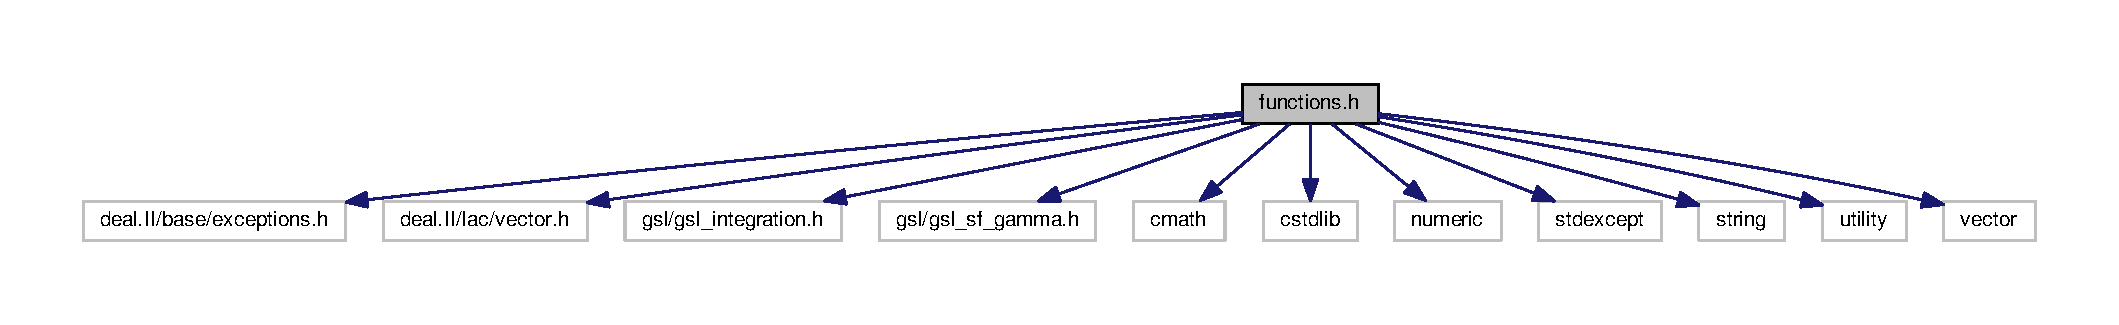
\includegraphics[width=350pt]{functions_8h__incl}
\end{center}
\end{figure}
This graph shows which files directly or indirectly include this file\+:
\nopagebreak
\begin{figure}[H]
\begin{center}
\leavevmode
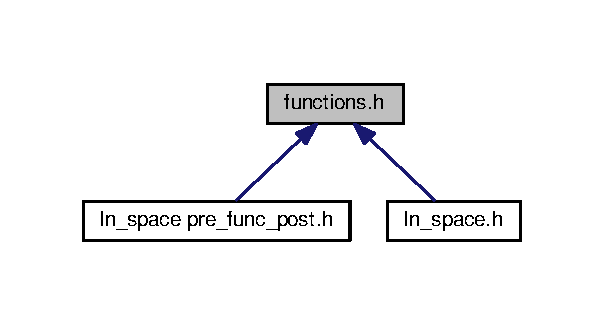
\includegraphics[width=145pt]{functions_8h__dep__incl}
\end{center}
\end{figure}
\subsection*{Macros}
\begin{DoxyCompactItemize}
\item 
\#define \hyperlink{functions_8h_a06d41b26246b319ff9d9b28be162b089}{outer\+\_\+product\+\_\+sym\+\_\+H}
\end{DoxyCompactItemize}
\subsection*{Functions}
\begin{DoxyCompactItemize}
\item 
{\footnotesize template$<$int dim$>$ }\\Tensor$<$ 4, dim $>$ \hyperlink{functions_8h_a6e649771188b6d625bea6309e77fbd16}{get\+\_\+tensor\+\_\+operator\+\_\+G} (const Symmetric\+Tensor$<$ 2, dim $>$ \&Ma, const Symmetric\+Tensor$<$ 2, dim $>$ \&Mb)
\item 
{\footnotesize template$<$int dim$>$ }\\Tensor$<$ 4, dim $>$ \hyperlink{functions_8h_acfd8da38df3766246f7bcf0e736ad9f4}{get\+\_\+tensor\+\_\+operator\+\_\+\+F\+\_\+right} (const Symmetric\+Tensor$<$ 2, dim $>$ \&Ma, const Symmetric\+Tensor$<$ 2, dim $>$ \&Mb, const Symmetric\+Tensor$<$ 2, dim $>$ \&Mc, const Symmetric\+Tensor$<$ 2, dim $>$ \&T)
\item 
{\footnotesize template$<$int dim$>$ }\\Tensor$<$ 4, dim $>$ \hyperlink{functions_8h_a6f9435c7728281851248d3537c100e7d}{get\+\_\+tensor\+\_\+operator\+\_\+\+F\+\_\+left} (const Symmetric\+Tensor$<$ 2, dim $>$ \&Ma, const Symmetric\+Tensor$<$ 2, dim $>$ \&Mb, const Symmetric\+Tensor$<$ 2, dim $>$ \&Mc, const Symmetric\+Tensor$<$ 2, dim $>$ \&T)
\item 
{\footnotesize template$<$int dim$>$ }\\Symmetric\+Tensor$<$ 4, dim $>$ \hyperlink{functions_8h_aa5f33021df9244e49e86b17b15286fa1}{outer\+\_\+product\+\_\+sym} (const Symmetric\+Tensor$<$ 2, dim $>$ \&A, const Symmetric\+Tensor$<$ 2, dim $>$ \&B)
\item 
{\footnotesize template$<$int dim$>$ }\\Symmetric\+Tensor$<$ 4, dim $>$ \hyperlink{functions_8h_a47630aad94c5f95af31f98cec5c0ec9a}{outer\+\_\+product\+\_\+sym} (const Symmetric\+Tensor$<$ 2, dim $>$ \&A)
\item 
{\footnotesize template$<$int dim$>$ }\\Symmetric\+Tensor$<$ 2, dim $>$ \hyperlink{functions_8h_a0ec7a717b44c3db05eb93bc370cca48c}{outer\+\_\+product\+\_\+sym} (const Tensor$<$ 1, dim $>$ \&A)
\item 
{\footnotesize template$<$int dim$>$ }\\bool \hyperlink{functions_8h_aa37f13547b984cb066e2fcb530b36425}{symmetry\+\_\+check} (Tensor$<$ 2, dim $>$ \&tensor)
\item 
{\footnotesize template$<$int dim$>$ }\\bool \hyperlink{functions_8h_adaf42311602a831f5c8c0fffdbb8aa63}{symmetry\+\_\+check} (const Tensor$<$ 4, dim $>$ \&temp)
\item 
{\footnotesize template$<$int dim$>$ }\\Symmetric\+Tensor$<$ 4, dim $>$ \hyperlink{functions_8h_afe83e9509497294b7f662b800b6b91ff}{symmetrize} (const Tensor$<$ 4, dim $>$ \&tensor)
\end{DoxyCompactItemize}


\subsection{Macro Definition Documentation}
\index{functions.\+h@{functions.\+h}!outer\+\_\+product\+\_\+sym\+\_\+H@{outer\+\_\+product\+\_\+sym\+\_\+H}}
\index{outer\+\_\+product\+\_\+sym\+\_\+H@{outer\+\_\+product\+\_\+sym\+\_\+H}!functions.\+h@{functions.\+h}}
\subsubsection[{\texorpdfstring{outer\+\_\+product\+\_\+sym\+\_\+H}{outer_product_sym_H}}]{\setlength{\rightskip}{0pt plus 5cm}\#define outer\+\_\+product\+\_\+sym\+\_\+H}\hypertarget{functions_8h_a06d41b26246b319ff9d9b28be162b089}{}\label{functions_8h_a06d41b26246b319ff9d9b28be162b089}


\subsection{Function Documentation}
\index{functions.\+h@{functions.\+h}!get\+\_\+tensor\+\_\+operator\+\_\+\+F\+\_\+left@{get\+\_\+tensor\+\_\+operator\+\_\+\+F\+\_\+left}}
\index{get\+\_\+tensor\+\_\+operator\+\_\+\+F\+\_\+left@{get\+\_\+tensor\+\_\+operator\+\_\+\+F\+\_\+left}!functions.\+h@{functions.\+h}}
\subsubsection[{\texorpdfstring{get\+\_\+tensor\+\_\+operator\+\_\+\+F\+\_\+left(const Symmetric\+Tensor$<$ 2, dim $>$ \&\+Ma, const Symmetric\+Tensor$<$ 2, dim $>$ \&\+Mb, const Symmetric\+Tensor$<$ 2, dim $>$ \&\+Mc, const Symmetric\+Tensor$<$ 2, dim $>$ \&\+T)}{get_tensor_operator_F_left(const SymmetricTensor< 2, dim > &Ma, const SymmetricTensor< 2, dim > &Mb, const SymmetricTensor< 2, dim > &Mc, const SymmetricTensor< 2, dim > &T)}}]{\setlength{\rightskip}{0pt plus 5cm}template$<$int dim$>$ Tensor$<$4,dim$>$ get\+\_\+tensor\+\_\+operator\+\_\+\+F\+\_\+left (
\begin{DoxyParamCaption}
\item[{const Symmetric\+Tensor$<$ 2, dim $>$ \&}]{Ma, }
\item[{const Symmetric\+Tensor$<$ 2, dim $>$ \&}]{Mb, }
\item[{const Symmetric\+Tensor$<$ 2, dim $>$ \&}]{Mc, }
\item[{const Symmetric\+Tensor$<$ 2, dim $>$ \&}]{T}
\end{DoxyParamCaption}
)}\hypertarget{functions_8h_a6f9435c7728281851248d3537c100e7d}{}\label{functions_8h_a6f9435c7728281851248d3537c100e7d}


Referenced by ln\+\_\+space$<$ dim $>$\+::post\+\_\+ln().


\begin{DoxyCode}
82                                                                          \{
83     Tensor<4,dim> tmp;
84 
85     Tensor<2,dim> temp\_tensor = contract<1,0>((Tensor<2,dim>)T, (Tensor<2,dim>)Mb);
86     Tensor<2,dim> MaTMb = contract<1,0>((Tensor<2,dim>)Ma,temp\_tensor);
87 
88     for(\textcolor{keywordtype}{unsigned} \textcolor{keywordtype}{int} i=0; i<dim; ++i)
89         for(\textcolor{keywordtype}{unsigned} \textcolor{keywordtype}{int} j=0; j<dim; ++j)
90             for(\textcolor{keywordtype}{unsigned} \textcolor{keywordtype}{int} k=0; k<dim; ++k)
91                 for(\textcolor{keywordtype}{unsigned} \textcolor{keywordtype}{int} l=k; l<dim; ++l)
92                 \{
93                     \textcolor{keywordtype}{double} tmp\_scalar = MaTMb[i][k] * Mc[j][l] + MaTMb[i][l] * Mc[j][k];
94                     tmp[i][j][k][l] = tmp\_scalar;
95                     tmp[i][j][l][k] = tmp\_scalar;
96                 \}
97 
98     \textcolor{keywordflow}{return} tmp;
99 \}
\end{DoxyCode}
\index{functions.\+h@{functions.\+h}!get\+\_\+tensor\+\_\+operator\+\_\+\+F\+\_\+right@{get\+\_\+tensor\+\_\+operator\+\_\+\+F\+\_\+right}}
\index{get\+\_\+tensor\+\_\+operator\+\_\+\+F\+\_\+right@{get\+\_\+tensor\+\_\+operator\+\_\+\+F\+\_\+right}!functions.\+h@{functions.\+h}}
\subsubsection[{\texorpdfstring{get\+\_\+tensor\+\_\+operator\+\_\+\+F\+\_\+right(const Symmetric\+Tensor$<$ 2, dim $>$ \&\+Ma, const Symmetric\+Tensor$<$ 2, dim $>$ \&\+Mb, const Symmetric\+Tensor$<$ 2, dim $>$ \&\+Mc, const Symmetric\+Tensor$<$ 2, dim $>$ \&\+T)}{get_tensor_operator_F_right(const SymmetricTensor< 2, dim > &Ma, const SymmetricTensor< 2, dim > &Mb, const SymmetricTensor< 2, dim > &Mc, const SymmetricTensor< 2, dim > &T)}}]{\setlength{\rightskip}{0pt plus 5cm}template$<$int dim$>$ Tensor$<$4,dim$>$ get\+\_\+tensor\+\_\+operator\+\_\+\+F\+\_\+right (
\begin{DoxyParamCaption}
\item[{const Symmetric\+Tensor$<$ 2, dim $>$ \&}]{Ma, }
\item[{const Symmetric\+Tensor$<$ 2, dim $>$ \&}]{Mb, }
\item[{const Symmetric\+Tensor$<$ 2, dim $>$ \&}]{Mc, }
\item[{const Symmetric\+Tensor$<$ 2, dim $>$ \&}]{T}
\end{DoxyParamCaption}
)}\hypertarget{functions_8h_acfd8da38df3766246f7bcf0e736ad9f4}{}\label{functions_8h_acfd8da38df3766246f7bcf0e736ad9f4}


Referenced by ln\+\_\+space$<$ dim $>$\+::post\+\_\+ln().


\begin{DoxyCode}
57 \{
58     Tensor<4,dim> tmp; \textcolor{comment}{// has minor symmetry of indices k,l}
59 
60     Tensor<2,dim> temp\_tensor = contract<1,0>((Tensor<2,dim>)T, (Tensor<2,dim>)Mc);
61     Tensor<2,dim> MbTMc = contract<1,0>((Tensor<2,dim>)Mb,temp\_tensor);
62 
63     for(\textcolor{keywordtype}{unsigned} \textcolor{keywordtype}{int} i=0; i<dim; ++i)
64         for(\textcolor{keywordtype}{unsigned} \textcolor{keywordtype}{int} j=0; j<dim; ++j)
65             for(\textcolor{keywordtype}{unsigned} \textcolor{keywordtype}{int} k=0; k<dim; ++k)
66                 for(\textcolor{keywordtype}{unsigned} \textcolor{keywordtype}{int} l=k; l<dim; ++l)
67                 \{
68                     \textcolor{keywordtype}{double} tmp\_scalar = Ma[i][k] * MbTMc[j][l] + Ma[i][l] * MbTMc[j][k];
69                     tmp[i][j][k][l] = tmp\_scalar;
70                     tmp[i][j][l][k] = tmp\_scalar;
71                 \}
72 
73     \textcolor{keywordflow}{return} tmp;
74 \}
\end{DoxyCode}
\index{functions.\+h@{functions.\+h}!get\+\_\+tensor\+\_\+operator\+\_\+G@{get\+\_\+tensor\+\_\+operator\+\_\+G}}
\index{get\+\_\+tensor\+\_\+operator\+\_\+G@{get\+\_\+tensor\+\_\+operator\+\_\+G}!functions.\+h@{functions.\+h}}
\subsubsection[{\texorpdfstring{get\+\_\+tensor\+\_\+operator\+\_\+\+G(const Symmetric\+Tensor$<$ 2, dim $>$ \&\+Ma, const Symmetric\+Tensor$<$ 2, dim $>$ \&\+Mb)}{get_tensor_operator_G(const SymmetricTensor< 2, dim > &Ma, const SymmetricTensor< 2, dim > &Mb)}}]{\setlength{\rightskip}{0pt plus 5cm}template$<$int dim$>$ Tensor$<$4,dim$>$ get\+\_\+tensor\+\_\+operator\+\_\+G (
\begin{DoxyParamCaption}
\item[{const Symmetric\+Tensor$<$ 2, dim $>$ \&}]{Ma, }
\item[{const Symmetric\+Tensor$<$ 2, dim $>$ \&}]{Mb}
\end{DoxyParamCaption}
)}\hypertarget{functions_8h_a6e649771188b6d625bea6309e77fbd16}{}\label{functions_8h_a6e649771188b6d625bea6309e77fbd16}


Referenced by ln\+\_\+space$<$ dim $>$\+::post\+\_\+ln().


\begin{DoxyCode}
34 \{
35     Tensor<4,dim> tmp; \textcolor{comment}{// has minor symmetry of indices k,l}
36 
37     \textcolor{keywordflow}{for}(\textcolor{keywordtype}{unsigned} \textcolor{keywordtype}{int} i=0; i<dim; ++i)
38         \textcolor{keywordflow}{for}(\textcolor{keywordtype}{unsigned} \textcolor{keywordtype}{int} j=0; j<dim; ++j)
39             \textcolor{keywordflow}{for}(\textcolor{keywordtype}{unsigned} \textcolor{keywordtype}{int} k=0; k<dim; ++k)
40                 \textcolor{keywordflow}{for}(\textcolor{keywordtype}{unsigned} \textcolor{keywordtype}{int} l=k; l<dim; ++l)
41                 \{
42                     \textcolor{keywordtype}{double} tmp\_scalar = Ma[i][k] * Mb[j][l] + Ma[i][l] * Mb[j][k];
43                     tmp[i][j][k][l] = tmp\_scalar;
44                     tmp[i][j][l][k] = tmp\_scalar;
45                 \}
46 
47     \textcolor{keywordflow}{return} tmp;
48 \}
\end{DoxyCode}
\index{functions.\+h@{functions.\+h}!outer\+\_\+product\+\_\+sym@{outer\+\_\+product\+\_\+sym}}
\index{outer\+\_\+product\+\_\+sym@{outer\+\_\+product\+\_\+sym}!functions.\+h@{functions.\+h}}
\subsubsection[{\texorpdfstring{outer\+\_\+product\+\_\+sym(const Symmetric\+Tensor$<$ 2, dim $>$ \&\+A, const Symmetric\+Tensor$<$ 2, dim $>$ \&\+B)}{outer_product_sym(const SymmetricTensor< 2, dim > &A, const SymmetricTensor< 2, dim > &B)}}]{\setlength{\rightskip}{0pt plus 5cm}template$<$int dim$>$ Symmetric\+Tensor$<$4,dim$>$ outer\+\_\+product\+\_\+sym (
\begin{DoxyParamCaption}
\item[{const Symmetric\+Tensor$<$ 2, dim $>$ \&}]{A, }
\item[{const Symmetric\+Tensor$<$ 2, dim $>$ \&}]{B}
\end{DoxyParamCaption}
)}\hypertarget{functions_8h_aa5f33021df9244e49e86b17b15286fa1}{}\label{functions_8h_aa5f33021df9244e49e86b17b15286fa1}


Referenced by ln\+\_\+space$<$ dim $>$\+::plastic\+\_\+right\+\_\+cauchy\+\_\+green\+\_\+\+A\+S(), ln\+\_\+space$<$ dim $>$\+::post\+\_\+ln(), and ln\+\_\+space$<$ dim $>$\+::pre\+\_\+ln().


\begin{DoxyCode}
111 \{
112     SymmetricTensor<4,dim> D;
113     \textcolor{comment}{// Special nested for-loop to access only non-symmetric entries of 4th order sym. tensor}
114     \textcolor{comment}{// ToDo: still not optimal element 1112 and 1211 are both accessed}
115     \textcolor{keywordflow}{for} ( \textcolor{keywordtype}{unsigned} \textcolor{keywordtype}{int} i=0; i<dim; ++i )
116         \textcolor{keywordflow}{for} ( \textcolor{keywordtype}{unsigned} \textcolor{keywordtype}{int} j=i; j<dim; ++j )
117             \textcolor{keywordflow}{for} ( \textcolor{keywordtype}{unsigned} \textcolor{keywordtype}{int} k=i; k<dim; ++k )
118                 \textcolor{keywordflow}{for} ( \textcolor{keywordtype}{unsigned} \textcolor{keywordtype}{int} l=k; l<dim; ++l )
119                 \{
120                     \textcolor{keywordtype}{double} tmp = A[i][j] * B[k][l] + B[i][j] * A[k][l];
121                     D[i][j][k][l] = tmp;
122                     D[k][l][i][j] = tmp;
123                 \}
124     \textcolor{keywordflow}{return} D;
125 \}
\end{DoxyCode}
\index{functions.\+h@{functions.\+h}!outer\+\_\+product\+\_\+sym@{outer\+\_\+product\+\_\+sym}}
\index{outer\+\_\+product\+\_\+sym@{outer\+\_\+product\+\_\+sym}!functions.\+h@{functions.\+h}}
\subsubsection[{\texorpdfstring{outer\+\_\+product\+\_\+sym(const Symmetric\+Tensor$<$ 2, dim $>$ \&\+A)}{outer_product_sym(const SymmetricTensor< 2, dim > &A)}}]{\setlength{\rightskip}{0pt plus 5cm}template$<$int dim$>$ Symmetric\+Tensor$<$4,dim$>$ outer\+\_\+product\+\_\+sym (
\begin{DoxyParamCaption}
\item[{const Symmetric\+Tensor$<$ 2, dim $>$ \&}]{A}
\end{DoxyParamCaption}
)}\hypertarget{functions_8h_a47630aad94c5f95af31f98cec5c0ec9a}{}\label{functions_8h_a47630aad94c5f95af31f98cec5c0ec9a}

\begin{DoxyCode}
128 \{
129     SymmetricTensor<4,dim> D;
130     \textcolor{comment}{// Special nested for-loop to access only non-symmetric entries of 4th order sym. tensor}
131     \textcolor{comment}{// ToDo: still not optimal element 1112 and 1211 are both accessed}
132     \textcolor{keywordflow}{for} ( \textcolor{keywordtype}{unsigned} \textcolor{keywordtype}{int} i=0; i<dim; ++i )
133         \textcolor{keywordflow}{for} ( \textcolor{keywordtype}{unsigned} \textcolor{keywordtype}{int} j=i; j<dim; ++j )
134             \textcolor{keywordflow}{for} ( \textcolor{keywordtype}{unsigned} \textcolor{keywordtype}{int} k=i; k<dim; ++k )
135                 \textcolor{keywordflow}{for} ( \textcolor{keywordtype}{unsigned} \textcolor{keywordtype}{int} l=k; l<dim; ++l )
136                 \{
137                     \textcolor{keywordtype}{double} tmp = A[i][j] * A[k][l];
138                     D[i][j][k][l] = tmp;
139                     D[k][l][i][j] = tmp;
140                 \}
141     \textcolor{keywordflow}{return} D;
142 \}
\end{DoxyCode}
\index{functions.\+h@{functions.\+h}!outer\+\_\+product\+\_\+sym@{outer\+\_\+product\+\_\+sym}}
\index{outer\+\_\+product\+\_\+sym@{outer\+\_\+product\+\_\+sym}!functions.\+h@{functions.\+h}}
\subsubsection[{\texorpdfstring{outer\+\_\+product\+\_\+sym(const Tensor$<$ 1, dim $>$ \&\+A)}{outer_product_sym(const Tensor< 1, dim > &A)}}]{\setlength{\rightskip}{0pt plus 5cm}template$<$int dim$>$ Symmetric\+Tensor$<$2,dim$>$ outer\+\_\+product\+\_\+sym (
\begin{DoxyParamCaption}
\item[{const Tensor$<$ 1, dim $>$ \&}]{A}
\end{DoxyParamCaption}
)}\hypertarget{functions_8h_a0ec7a717b44c3db05eb93bc370cca48c}{}\label{functions_8h_a0ec7a717b44c3db05eb93bc370cca48c}

\begin{DoxyCode}
145 \{
146     SymmetricTensor<2,dim> D;
147     \textcolor{comment}{// Special nested for-loop to access only non-symmetric entries of 4th order sym. tensor}
148     \textcolor{comment}{// ToDo: still not optimal element 1112 and 1211 are both accessed}
149     \textcolor{keywordflow}{for} ( \textcolor{keywordtype}{unsigned} \textcolor{keywordtype}{int} i=0; i<dim; ++i )
150         \textcolor{keywordflow}{for} ( \textcolor{keywordtype}{unsigned} \textcolor{keywordtype}{int} j=i; j<dim; ++j )
151             D[i][j] = A[i] * A[j];
152 
153     \textcolor{keywordflow}{return} D;
154 \}
\end{DoxyCode}
\index{functions.\+h@{functions.\+h}!symmetrize@{symmetrize}}
\index{symmetrize@{symmetrize}!functions.\+h@{functions.\+h}}
\subsubsection[{\texorpdfstring{symmetrize(const Tensor$<$ 4, dim $>$ \&tensor)}{symmetrize(const Tensor< 4, dim > &tensor)}}]{\setlength{\rightskip}{0pt plus 5cm}template$<$int dim$>$ Symmetric\+Tensor$<$4,dim$>$ symmetrize (
\begin{DoxyParamCaption}
\item[{const Tensor$<$ 4, dim $>$ \&}]{tensor}
\end{DoxyParamCaption}
)}\hypertarget{functions_8h_afe83e9509497294b7f662b800b6b91ff}{}\label{functions_8h_afe83e9509497294b7f662b800b6b91ff}


References symmetry\+\_\+check().



Referenced by ln\+\_\+space$<$ dim $>$\+::post\+\_\+ln(), and ln\+\_\+space$<$ dim $>$\+::pre\+\_\+ln().


\begin{DoxyCode}
209                                                               \{
210     SymmetricTensor<4,dim> sym\_tensor;
211     Assert(\hyperlink{functions_8h_aa37f13547b984cb066e2fcb530b36425}{symmetry\_check}(tensor), ExcMessage(\textcolor{stringliteral}{"Tensor to symmetrize is not symmetric!"}));
212 
213     Tensor<4,dim> temp\_tensor;
214     \textcolor{keywordflow}{for}(\textcolor{keywordtype}{unsigned} \textcolor{keywordtype}{int} i=0; i<dim; ++i)
215         \textcolor{keywordflow}{for}(\textcolor{keywordtype}{unsigned} \textcolor{keywordtype}{int} j=0; j<dim; ++j)
216             \textcolor{keywordflow}{for}(\textcolor{keywordtype}{unsigned} \textcolor{keywordtype}{int} k=0; k<dim; ++k)
217                 \textcolor{keywordflow}{for}(\textcolor{keywordtype}{unsigned} \textcolor{keywordtype}{int} l=0; l<dim; ++l)
218                     temp\_tensor[i][j][k][l] = (tensor[i][j][k][l]+tensor[j][i][k][l]+tensor[i][j][l][k]) / 
      3.0;
219 
220     \textcolor{keywordflow}{for}(\textcolor{keywordtype}{unsigned} \textcolor{keywordtype}{int} i=0; i<dim; ++i)
221         \textcolor{keywordflow}{for}(\textcolor{keywordtype}{unsigned} \textcolor{keywordtype}{int} j=i; j<dim; ++j)
222             \textcolor{keywordflow}{for}(\textcolor{keywordtype}{unsigned} \textcolor{keywordtype}{int} k=0; k<dim; ++k)
223                 \textcolor{keywordflow}{for}(\textcolor{keywordtype}{unsigned} \textcolor{keywordtype}{int} l=k; l<dim; ++l)
224                     sym\_tensor[i][j][k][l] = temp\_tensor[i][j][k][l];
225 \textcolor{comment}{//                    sym\_tensor[i][j][k][l] = tensor[i][j][k][l];}
226 
227     \textcolor{keywordflow}{return} sym\_tensor;
228 \}
\end{DoxyCode}
\index{functions.\+h@{functions.\+h}!symmetry\+\_\+check@{symmetry\+\_\+check}}
\index{symmetry\+\_\+check@{symmetry\+\_\+check}!functions.\+h@{functions.\+h}}
\subsubsection[{\texorpdfstring{symmetry\+\_\+check(\+Tensor$<$ 2, dim $>$ \&tensor)}{symmetry_check(Tensor< 2, dim > &tensor)}}]{\setlength{\rightskip}{0pt plus 5cm}template$<$int dim$>$ bool symmetry\+\_\+check (
\begin{DoxyParamCaption}
\item[{Tensor$<$ 2, dim $>$ \&}]{tensor}
\end{DoxyParamCaption}
)}\hypertarget{functions_8h_aa37f13547b984cb066e2fcb530b36425}{}\label{functions_8h_aa37f13547b984cb066e2fcb530b36425}


Referenced by ln\+\_\+space$<$ dim $>$\+::post\+\_\+ln(), and symmetrize().


\begin{DoxyCode}
164 \{
165     \textcolor{keywordflow}{for} ( \textcolor{keywordtype}{unsigned} \textcolor{keywordtype}{int} i=0; i<dim; i++ )
166         \textcolor{keywordflow}{for} ( \textcolor{keywordtype}{unsigned} \textcolor{keywordtype}{int} j=0; j<dim; j++ )
167             \textcolor{keywordflow}{if} ( i!=j && ( std::abs(tensor[i][j] - tensor[j][i])>1e-12 ) )
168                 \textcolor{keywordflow}{return} \textcolor{keyword}{false};
169 
170     \textcolor{keywordflow}{return} \textcolor{keyword}{true};
171 \}
\end{DoxyCode}
\index{functions.\+h@{functions.\+h}!symmetry\+\_\+check@{symmetry\+\_\+check}}
\index{symmetry\+\_\+check@{symmetry\+\_\+check}!functions.\+h@{functions.\+h}}
\subsubsection[{\texorpdfstring{symmetry\+\_\+check(const Tensor$<$ 4, dim $>$ \&temp)}{symmetry_check(const Tensor< 4, dim > &temp)}}]{\setlength{\rightskip}{0pt plus 5cm}template$<$int dim$>$ bool symmetry\+\_\+check (
\begin{DoxyParamCaption}
\item[{const Tensor$<$ 4, dim $>$ \&}]{temp}
\end{DoxyParamCaption}
)}\hypertarget{functions_8h_adaf42311602a831f5c8c0fffdbb8aa63}{}\label{functions_8h_adaf42311602a831f5c8c0fffdbb8aa63}

\begin{DoxyCode}
173                                               \{
174     \textcolor{keywordflow}{for}(\textcolor{keywordtype}{unsigned} \textcolor{keywordtype}{int} i=0; i<dim; ++i)\{
175         \textcolor{keywordflow}{for}(\textcolor{keywordtype}{unsigned} \textcolor{keywordtype}{int} j=0; j<dim; ++j)\{
176             \textcolor{keywordflow}{for}(\textcolor{keywordtype}{unsigned} \textcolor{keywordtype}{int} k=0; k<dim; ++k)\{
177                 \textcolor{keywordflow}{for}(\textcolor{keywordtype}{unsigned} \textcolor{keywordtype}{int} l=0; l<dim; ++l)\{
178                     \textcolor{comment}{// absolute difference check}
179                     \textcolor{keywordflow}{if}(    ( fabs(temp[i][j][k][l] - temp[j][i][k][l]) > 1e-6 )
180                             ||
181                           ( fabs(temp[i][j][k][l] - temp[i][j][l][k]) > 1e-6 ) )
182                     \{
183                         \textcolor{comment}{// relative difference check}
184                         \textcolor{keywordflow}{if}( (fabs(fabs(temp[i][j][k][l] - temp[j][i][k][l])/temp[j][i][k][l])> 1e-8)
185                             ||
186                           (fabs(fabs(temp[i][j][k][l] - temp[i][j][l][k])/temp[i][j][l][k]) >1e-8) )
187                         \{
188                             deallog<< std::endl;
189                             deallog<< \textcolor{stringliteral}{"Abs not matching: "}<<fabs(temp[i][j][k][l] - temp[j][i][k][l])
190                                 << \textcolor{stringliteral}{" | Rel not matching: "}<<fabs(temp[i][j][k][l] - temp[j][i][k][l])/temp[
      j][i][k][l]
191                                 << \textcolor{stringliteral}{" | Abs not matching: "}<<fabs(temp[i][j][k][l] - temp[i][j][l][k])
192                                 << \textcolor{stringliteral}{" | Rel not matching: "}<<fabs(temp[i][j][k][l] - temp[i][j][l][k])/temp[
      i][j][l][k]
193                                 << \textcolor{stringliteral}{" | value ijkl: "}<< std::scientific << temp[i][j][k][l]
194                                 << \textcolor{stringliteral}{" | value jikl: "}<< std::scientific << temp[j][i][k][l]
195                                 << \textcolor{stringliteral}{" | value ijlk: "}<< std::scientific << temp[i][j][l][k]
196                                 << std::endl;
197                             \textcolor{keywordflow}{return} \textcolor{keyword}{false};
198                         \}
199                     \}
200                 \}
201             \}
202         \}
203     \}
204     \textcolor{keywordflow}{return} \textcolor{keyword}{true};
205 \}
\end{DoxyCode}

\hypertarget{ln__space_8h}{}\section{ln\+\_\+space.\+h File Reference}
\label{ln__space_8h}\index{ln\+\_\+space.\+h@{ln\+\_\+space.\+h}}
{\ttfamily \#include $<$deal.\+I\+I/base/symmetric\+\_\+tensor.\+h$>$}\\*
{\ttfamily \#include $<$deal.\+I\+I/base/exceptions.\+h$>$}\\*
{\ttfamily \#include $<$iostream$>$}\\*
{\ttfamily \#include $<$fstream$>$}\\*
{\ttfamily \#include $<$cmath$>$}\\*
{\ttfamily \#include \char`\"{}functions.\+h\char`\"{}}\\*
Include dependency graph for ln\+\_\+space.\+h\+:\nopagebreak
\begin{figure}[H]
\begin{center}
\leavevmode
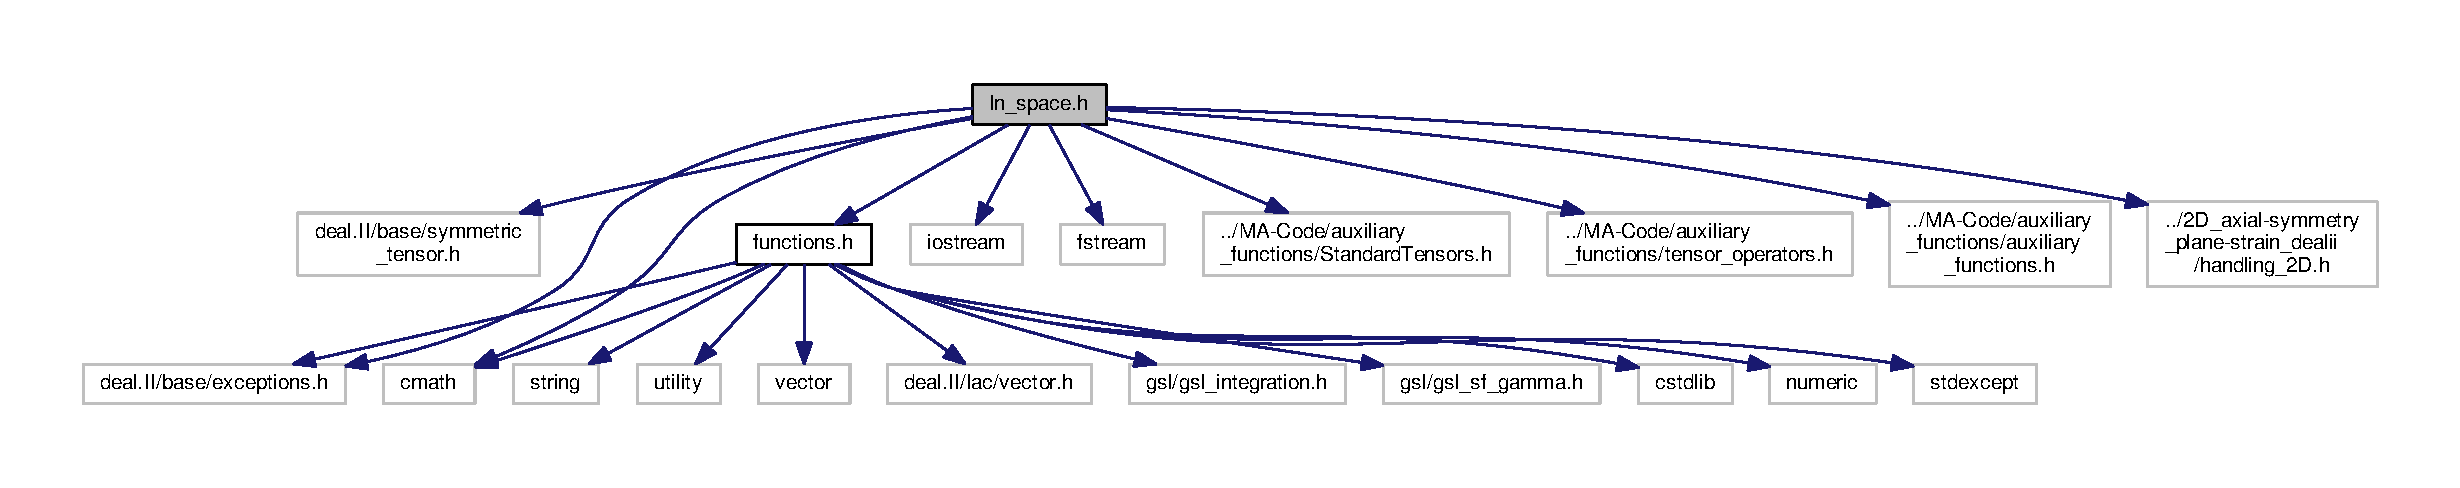
\includegraphics[width=350pt]{ln__space_8h__incl}
\end{center}
\end{figure}
\subsection*{Namespaces}
\begin{DoxyCompactItemize}
\item 
 \hyperlink{namespaceln__space}{ln\+\_\+space}
\end{DoxyCompactItemize}
\subsection*{Functions}
\begin{DoxyCompactItemize}
\item 
{\footnotesize template$<$int dim$>$ }\\void \hyperlink{namespaceln__space_a85e361462746b126386ad7e1d608e7d8}{ln\+\_\+space\+::pre\+\_\+ln} (Tensor$<$ 2, dim $>$ \&F, Symmetric\+Tensor$<$ 2, dim $>$ \&hencky\+\_\+strain, Vector$<$ double $>$ \&ea, Vector$<$ double $>$ \&da, Vector$<$ double $>$ \&fa, std\+::vector$<$ Tensor$<$ 1, dim $>$ $>$ \&eigenvector, Vector$<$ double $>$ \&eigenvalues, std\+::vector$<$ Symmetric\+Tensor$<$ 2, dim $>$ $>$ \&eigenbasis)
\item 
{\footnotesize template$<$int dim$>$ }\\void \hyperlink{namespaceln__space_a0f5e3bde0b1ee47f3dbc5977b4653342}{ln\+\_\+space\+::post\+\_\+ln} (Vector$<$ double $>$ \&ea, Vector$<$ double $>$ \&da, Vector$<$ double $>$ \&fa, Vector$<$ double $>$ \&eigenvalues, std\+::vector$<$ Symmetric\+Tensor$<$ 2, dim $>$ $>$ \&eigenbasis, Symmetric\+Tensor$<$ 2, dim $>$ \&second\+\_\+piola\+\_\+stress\+\_\+S, Symmetric\+Tensor$<$ 4, dim $>$ \&elasto\+\_\+plastic\+\_\+tangent)
\end{DoxyCompactItemize}

\hypertarget{mainpage_8h}{}\section{mainpage.\+h File Reference}
\label{mainpage_8h}\index{mainpage.\+h@{mainpage.\+h}}

\hypertarget{README_8md}{}\section{R\+E\+A\+D\+M\+E.\+md File Reference}
\label{README_8md}\index{R\+E\+A\+D\+M\+E.\+md@{R\+E\+A\+D\+M\+E.\+md}}

%--- End generated contents ---

% Index
\backmatter
\newpage
\phantomsection
\clearemptydoublepage
\addcontentsline{toc}{chapter}{Index}
\printindex

\end{document}
